\chapter{The Specific Heat of Helium-4 and Godfrin's Series}\label{ch04}
% generated by figures/ch04_numbers_tex.py from figures/ch04_numbers.json -- do not edit
\makeatletter
\providecommand{\cfv}[1]{\ifcsname cfv@#1\endcsname\csname cfv@#1\endcsname\else\PackageError{ch04}{Undefined number key #1}{Run ch04_numbers_tex.py}\fi}
\expandafter\gdef\csname cfv@A-pr\endcsname{\ensuremath{0.0831}}
\expandafter\gdef\csname cfv@A-val\endcsname{\ensuremath{0.083091}}
\expandafter\gdef\csname cfv@C-pr\endcsname{\ensuremath{-0.0548}}
\expandafter\gdef\csname cfv@C-val\endcsname{\ensuremath{-0.054809}}
\expandafter\gdef\csname cfv@D-pr\endcsname{\ensuremath{0.0653}}
\expandafter\gdef\csname cfv@D-val\endcsname{\ensuremath{0.065345}}
\expandafter\gdef\csname cfv@E-pr\endcsname{\ensuremath{0.0603}}
\expandafter\gdef\csname cfv@E-val\endcsname{\ensuremath{0.060370}}
\expandafter\gdef\csname cfv@K-pr\endcsname{\ensuremath{-0.262}}
\expandafter\gdef\csname cfv@K-val\endcsname{\ensuremath{-0.26247}}
\expandafter\gdef\csname cfv@L-pr\endcsname{\ensuremath{0.141}}
\expandafter\gdef\csname cfv@L-val\endcsname{\ensuremath{0.14086}}
\expandafter\gdef\csname cfv@T-cross\endcsname{0.77}
\expandafter\gdef\csname cfv@Trange-hi-A\endcsname{0.0543}
\expandafter\gdef\csname cfv@Trange-hi-AC\endcsname{0.0543}
\expandafter\gdef\csname cfv@Trange-hi-ACD\endcsname{0.0543}
\expandafter\gdef\csname cfv@Trange-hi-ACDE\endcsname{0.0543}
\expandafter\gdef\csname cfv@Trange-hi-ACDEK\endcsname{0.0543}
\expandafter\gdef\csname cfv@Trange-hi-ACDEKL\endcsname{0.0543}
\expandafter\gdef\csname cfv@Trange-lo-A\endcsname{0.005}
\expandafter\gdef\csname cfv@Trange-lo-AC\endcsname{0.005}
\expandafter\gdef\csname cfv@Trange-lo-ACD\endcsname{0.005}
\expandafter\gdef\csname cfv@Trange-lo-ACDE\endcsname{0.00849}
\expandafter\gdef\csname cfv@Trange-lo-ACDEK\endcsname{0.0144}
\expandafter\gdef\csname cfv@Trange-lo-ACDEKL\endcsname{0.0188}
\expandafter\gdef\csname cfv@V\endcsname{27.5793}
\expandafter\gdef\csname cfv@a2\endcsname{1.55}
\expandafter\gdef\csname cfv@a3\endcsname{-4.04}
\expandafter\gdef\csname cfv@a4\endcsname{2.30}
\expandafter\gdef\csname cfv@best-err-0.2\endcsname{\ensuremath{2.8\times10^{-7}}}
\expandafter\gdef\csname cfv@best-err-0.3\endcsname{\ensuremath{1.3\times10^{-4}}}
\expandafter\gdef\csname cfv@best-err-0.5\endcsname{\ensuremath{7.6\times10^{-3}}}
\expandafter\gdef\csname cfv@best-err-0.8\endcsname{\ensuremath{9.1\times10^{-2}}}
\expandafter\gdef\csname cfv@best-order-0.2\endcsname{19}
\expandafter\gdef\csname cfv@best-order-0.3\endcsname{19}
\expandafter\gdef\csname cfv@best-order-0.5\endcsname{6}
\expandafter\gdef\csname cfv@best-order-0.8\endcsname{6}
\expandafter\gdef\csname cfv@bose-XEND\endcsname{80}
\expandafter\gdef\csname cfv@bose-calls-1m10\endcsname{688}
\expandafter\gdef\csname cfv@bose-calls-1m12\endcsname{848}
\expandafter\gdef\csname cfv@bose-calls-1m4\endcsname{231}
\expandafter\gdef\csname cfv@bose-calls-1m6\endcsname{383}
\expandafter\gdef\csname cfv@bose-calls-1m8\endcsname{528}
\expandafter\gdef\csname cfv@bose-err-1m10\endcsname{\ensuremath{3.3\times10^{-9}}}
\expandafter\gdef\csname cfv@bose-err-1m12\endcsname{\ensuremath{2.4\times10^{-11}}}
\expandafter\gdef\csname cfv@bose-err-1m4\endcsname{\ensuremath{5.1\times10^{-4}}}
\expandafter\gdef\csname cfv@bose-err-1m6\endcsname{\ensuremath{2.4\times10^{-5}}}
\expandafter\gdef\csname cfv@bose-err-1m8\endcsname{\ensuremath{2.0\times10^{-7}}}
\expandafter\gdef\csname cfv@bose-quad\endcsname{\ensuremath{1\times10^{-16}}}
\expandafter\gdef\csname cfv@bose-ratio-max\endcsname{33}
\expandafter\gdef\csname cfv@bose-ratio-min\endcsname{5.1}
\expandafter\gdef\csname cfv@bud-first_T_series6_vs_measured_ph_exceeds_1pct\endcsname{0.45}
\expandafter\gdef\csname cfv@bud-first_T_series6_vs_poly_exceeds_0p1pct\endcsname{0.30}
\expandafter\gdef\csname cfv@bud-first_T_series6_vs_poly_exceeds_1pct\endcsname{0.45}
\expandafter\gdef\csname cfv@bud-model-0.3\endcsname{\ensuremath{6.0\times10^{-4}}}
\expandafter\gdef\csname cfv@bud-model-0.4\endcsname{\ensuremath{9.8\times10^{-4}}}
\expandafter\gdef\csname cfv@bud-model-0.5\endcsname{\ensuremath{1.4\times10^{-3}}}
\expandafter\gdef\csname cfv@bud-model-0.6\endcsname{\ensuremath{1.7\times10^{-3}}}
\expandafter\gdef\csname cfv@bud-model-0.7\endcsname{\ensuremath{2.0\times10^{-3}}}
\expandafter\gdef\csname cfv@bud-model-0.8\endcsname{\ensuremath{1.8\times10^{-3}}}
\expandafter\gdef\csname cfv@bud-model-1.0\endcsname{\ensuremath{2.1\times10^{-3}}}
\expandafter\gdef\csname cfv@bud-model-pct-0.3\endcsname{0.06}
\expandafter\gdef\csname cfv@bud-model-pct-0.4\endcsname{0.098}
\expandafter\gdef\csname cfv@bud-model-pct-0.5\endcsname{0.14}
\expandafter\gdef\csname cfv@bud-model-pct-0.6\endcsname{0.17}
\expandafter\gdef\csname cfv@bud-model-pct-0.7\endcsname{0.2}
\expandafter\gdef\csname cfv@bud-model-pct-0.8\endcsname{0.18}
\expandafter\gdef\csname cfv@bud-model-pct-1.0\endcsname{0.21}
\expandafter\gdef\csname cfv@bud-tot-0.3\endcsname{\ensuremath{4.9\times10^{-4}}}
\expandafter\gdef\csname cfv@bud-tot-0.4\endcsname{\ensuremath{5.1\times10^{-3}}}
\expandafter\gdef\csname cfv@bud-tot-0.5\endcsname{\ensuremath{2.0\times10^{-2}}}
\expandafter\gdef\csname cfv@bud-tot-0.6\endcsname{\ensuremath{5.5\times10^{-2}}}
\expandafter\gdef\csname cfv@bud-tot-0.7\endcsname{\ensuremath{1.2\times10^{-1}}}
\expandafter\gdef\csname cfv@bud-tot-0.8\endcsname{\ensuremath{2.3\times10^{-1}}}
\expandafter\gdef\csname cfv@bud-tot-1.0\endcsname{\ensuremath{5.8\times10^{-1}}}
\expandafter\gdef\csname cfv@bud-tot-pct-0.3\endcsname{0.049}
\expandafter\gdef\csname cfv@bud-tot-pct-0.4\endcsname{0.51}
\expandafter\gdef\csname cfv@bud-tot-pct-0.5\endcsname{2}
\expandafter\gdef\csname cfv@bud-tot-pct-0.6\endcsname{5.5}
\expandafter\gdef\csname cfv@bud-tot-pct-0.7\endcsname{12}
\expandafter\gdef\csname cfv@bud-tot-pct-0.8\endcsname{23}
\expandafter\gdef\csname cfv@bud-tot-pct-1.0\endcsname{58}
\expandafter\gdef\csname cfv@bud-trunc-0.3\endcsname{\ensuremath{1.1\times10^{-3}}}
\expandafter\gdef\csname cfv@bud-trunc-0.4\endcsname{\ensuremath{6.0\times10^{-3}}}
\expandafter\gdef\csname cfv@bud-trunc-0.5\endcsname{\ensuremath{2.1\times10^{-2}}}
\expandafter\gdef\csname cfv@bud-trunc-0.6\endcsname{\ensuremath{5.7\times10^{-2}}}
\expandafter\gdef\csname cfv@bud-trunc-0.7\endcsname{\ensuremath{1.2\times10^{-1}}}
\expandafter\gdef\csname cfv@bud-trunc-0.8\endcsname{\ensuremath{2.4\times10^{-1}}}
\expandafter\gdef\csname cfv@bud-trunc-1.0\endcsname{\ensuremath{5.8\times10^{-1}}}
\expandafter\gdef\csname cfv@bud-trunc-pct-0.3\endcsname{0.11}
\expandafter\gdef\csname cfv@bud-trunc-pct-0.4\endcsname{0.6}
\expandafter\gdef\csname cfv@bud-trunc-pct-0.5\endcsname{2.1}
\expandafter\gdef\csname cfv@bud-trunc-pct-0.6\endcsname{5.7}
\expandafter\gdef\csname cfv@bud-trunc-pct-0.7\endcsname{12}
\expandafter\gdef\csname cfv@bud-trunc-pct-0.8\endcsname{24}
\expandafter\gdef\csname cfv@bud-trunc-pct-1.0\endcsname{58}
\expandafter\gdef\csname cfv@c\endcsname{238.3}
\expandafter\gdef\csname cfv@c10\endcsname{\ensuremath{1.039}}
\expandafter\gdef\csname cfv@c11\endcsname{\ensuremath{-2.585}}
\expandafter\gdef\csname cfv@cert-kSq0\endcsname{42}
\expandafter\gdef\csname cfv@cert-list\endcsname{202, 156, 116, 82, 58 and 40}
\expandafter\gdef\csname cfv@coef-maxdiff\endcsname{0.18}
\expandafter\gdef\csname cfv@ctl-D-0.05\endcsname{\ensuremath{6.5\times10^{-9}}}
\expandafter\gdef\csname cfv@ctl-D-0.1\endcsname{\ensuremath{5.2\times10^{-8}}}
\expandafter\gdef\csname cfv@ctl-D-ratio\endcsname{24}
\expandafter\gdef\csname cfv@ctl-D-rel\endcsname{\ensuremath{6.6\times10^{-5}}}
\expandafter\gdef\csname cfv@ctl-K-0.05\endcsname{\ensuremath{1.1\times10^{-7}}}
\expandafter\gdef\csname cfv@ctl-K-0.1\endcsname{\ensuremath{3.5\times10^{-6}}}
\expandafter\gdef\csname cfv@ctl-K-ratio\endcsname{2.8}
\expandafter\gdef\csname cfv@ctl-K-rel\endcsname{11}
\expandafter\gdef\csname cfv@ctl-L-0.1\endcsname{\ensuremath{4.3\times10^{-8}}}
\expandafter\gdef\csname cfv@ctl-L-ratio\endcsname{29}
\expandafter\gdef\csname cfv@ctl-L-rel\endcsname{2.5}
\expandafter\gdef\csname cfv@ctl-next-0.05\endcsname{\ensuremath{9.8\times10^{-9}}}
\expandafter\gdef\csname cfv@ctl-next-0.1\endcsname{\ensuremath{1.3\times10^{-6}}}
\expandafter\gdef\csname cfv@cv-0.1\endcsname{8.260\times10^{-5}}
\expandafter\gdef\csname cfv@cv-0.2\endcsname{6.513\times10^{-4}}
\expandafter\gdef\csname cfv@cv-ratio\endcsname{7.88}
\expandafter\gdef\csname cfv@cv-ratio-dev\endcsname{1.4}
\expandafter\gdef\csname cfv@cvT3-0.1\endcsname{0.0826}
\expandafter\gdef\csname cfv@cvT3-0.5\endcsname{0.0780}
\expandafter\gdef\csname cfv@cvT3-ph-0.1\endcsname{0.0826}
\expandafter\gdef\csname cfv@cvT3-ph-0.5\endcsname{0.0769}
\expandafter\gdef\csname cfv@err9-0.2\endcsname{\ensuremath{8.8\times10^{-5}}}
\expandafter\gdef\csname cfv@err9-0.3\endcsname{\ensuremath{1.1\times10^{-3}}}
\expandafter\gdef\csname cfv@err9-0.5\endcsname{\ensuremath{2.1\times10^{-2}}}
\expandafter\gdef\csname cfv@err9-0.8\endcsname{\ensuremath{2.4\times10^{-1}}}
\expandafter\gdef\csname cfv@fit-T-hi\endcsname{0.6}
\expandafter\gdef\csname cfv@fit-T-lo\endcsname{0.08}
\expandafter\gdef\csname cfv@fit-b\endcsname{\ensuremath{4.47}}
\expandafter\gdef\csname cfv@fit-b-pred\endcsname{\ensuremath{4.50}}
\expandafter\gdef\csname cfv@fit-s\endcsname{\ensuremath{-3.7}}
\expandafter\gdef\csname cfv@floor\endcsname{\ensuremath{4\times10^{-13}}}
\expandafter\gdef\csname cfv@floor-0.02\endcsname{\ensuremath{5\times10^{-15}}}
\expandafter\gdef\csname cfv@floor-0.1\endcsname{\ensuremath{4\times10^{-15}}}
\expandafter\gdef\csname cfv@grid-coarse\endcsname{0.05}
\expandafter\gdef\csname cfv@grid-until\endcsname{3.44}
\expandafter\gdef\csname cfv@kT\endcsname{\ensuremath{0.0549}}
\expandafter\gdef\csname cfv@lambda-0.1\endcsname{257}
\expandafter\gdef\csname cfv@lean-toolchain\endcsname{4.34.0-rc2}
\expandafter\gdef\csname cfv@maxdev-ueV\endcsname{2.2}
\expandafter\gdef\csname cfv@maxon-K\endcsname{13.8}
\expandafter\gdef\csname cfv@maxon-k\endcsname{1.114}
\expandafter\gdef\csname cfv@med-k-0.1\endcsname{0.024}
\expandafter\gdef\csname cfv@med-k-0.3\endcsname{0.072}
\expandafter\gdef\csname cfv@med-k-0.5\endcsname{0.119}
\expandafter\gdef\csname cfv@med-k-1.0\endcsname{1.881}
\expandafter\gdef\csname cfv@model-abserr\endcsname{\ensuremath{4\times10^{-13}}}
\expandafter\gdef\csname cfv@model-abserr-0.1\endcsname{\ensuremath{4\times10^{-15}}}
\expandafter\gdef\csname cfv@model-calls\endcsname{2\,370}
\expandafter\gdef\csname cfv@model-gain\endcsname{13}
\expandafter\gdef\csname cfv@model-load\endcsname{20}
\expandafter\gdef\csname cfv@model-raw-abserr\endcsname{\ensuremath{7\times10^{-12}}}
\expandafter\gdef\csname cfv@model-raw-abserr-0.1\endcsname{\ensuremath{5\times10^{-14}}}
\expandafter\gdef\csname cfv@model-seconds\endcsname{3}
\expandafter\gdef\csname cfv@n-T\endcsname{26}
\expandafter\gdef\csname cfv@n-err-rows\endcsname{34}
\expandafter\gdef\csname cfv@n-gaps\endcsname{4}
\expandafter\gdef\csname cfv@n-rows\endcsname{1727}
\expandafter\gdef\csname cfv@nT-all\endcsname{68}
\expandafter\gdef\csname cfv@nT-lin\endcsname{26}
\expandafter\gdef\csname cfv@nT-log\endcsname{41}
\expandafter\gdef\csname cfv@new-adams-bose-calls\endcsname{260}
\expandafter\gdef\csname cfv@new-adams-bose-err\endcsname{\ensuremath{2.8\times10^{-7}}}
\expandafter\gdef\csname cfv@new-adams-decay-calls\endcsname{511}
\expandafter\gdef\csname cfv@new-landing-err\endcsname{0}
\expandafter\gdef\csname cfv@old-adams-bose-calls\endcsname{15\,532}
\expandafter\gdef\csname cfv@old-adams-bose-err\endcsname{\ensuremath{6.5\times10^{-4}}}
\expandafter\gdef\csname cfv@old-adams-bose-ratio\endcsname{649}
\expandafter\gdef\csname cfv@old-adams-cos-t\endcsname{25}
\expandafter\gdef\csname cfv@old-adams-landing-cap\endcsname{0}
\expandafter\gdef\csname cfv@old-bdf-bose-calls\endcsname{413}
\expandafter\gdef\csname cfv@old-bdf-bose-err\endcsname{\ensuremath{1.3\times10^{-6}}}
\expandafter\gdef\csname cfv@old-bdf-landing-err\endcsname{38}
\expandafter\gdef\csname cfv@paper-unc-0.1\endcsname{0.13}
\expandafter\gdef\csname cfv@paper-unc-0.2\endcsname{0.17}
\expandafter\gdef\csname cfv@paper-unc-0.3\endcsname{0.26}
\expandafter\gdef\csname cfv@paper-unc-0.5\endcsname{0.38}
\expandafter\gdef\csname cfv@paper-unc-0.7\endcsname{0.86}
\expandafter\gdef\csname cfv@poly-dev-1\endcsname{7.6}
\expandafter\gdef\csname cfv@probe-cap\endcsname{60\,000}
\expandafter\gdef\csname cfv@probe-landing-n\endcsname{160}
\expandafter\gdef\csname cfv@pstar-0.1\endcsname{46}
\expandafter\gdef\csname cfv@pstar-0.15\endcsname{28}
\expandafter\gdef\csname cfv@pstar-0.2\endcsname{20}
\expandafter\gdef\csname cfv@pstar-0.3\endcsname{15}
\expandafter\gdef\csname cfv@pstar-0.4\endcsname{10}
\expandafter\gdef\csname cfv@pstar-0.5\endcsname{7}
\expandafter\gdef\csname cfv@pstar-pred-0.1\endcsname{45}
\expandafter\gdef\csname cfv@pstar-pred-0.15\endcsname{30}
\expandafter\gdef\csname cfv@pstar-pred-0.2\endcsname{23}
\expandafter\gdef\csname cfv@pstar-pred-0.3\endcsname{15}
\expandafter\gdef\csname cfv@pstar-pred-0.4\endcsname{11}
\expandafter\gdef\csname cfv@pstar-pred-0.5\endcsname{9}
\expandafter\gdef\csname cfv@q90-k-0.1\endcsname{0.043}
\expandafter\gdef\csname cfv@q90-k-0.3\endcsname{0.126}
\expandafter\gdef\csname cfv@q90-k-0.5\endcsname{0.211}
\expandafter\gdef\csname cfv@q90-k-1.0\endcsname{2.077}
\expandafter\gdef\csname cfv@rA-10\endcsname{\ensuremath{13}}
\expandafter\gdef\csname cfv@rA-11\endcsname{\ensuremath{-31}}
\expandafter\gdef\csname cfv@rA-12\endcsname{\ensuremath{-29}}
\expandafter\gdef\csname cfv@rA-13\endcsname{\ensuremath{313}}
\expandafter\gdef\csname cfv@rA-14\endcsname{\ensuremath{-399}}
\expandafter\gdef\csname cfv@rA-5\endcsname{\ensuremath{-0.66}}
\expandafter\gdef\csname cfv@rA-6\endcsname{\ensuremath{0.79}}
\expandafter\gdef\csname cfv@rA-7\endcsname{\ensuremath{0.73}}
\expandafter\gdef\csname cfv@rA-8\endcsname{\ensuremath{-3.16}}
\expandafter\gdef\csname cfv@rA-9\endcsname{\ensuremath{1.70}}
\expandafter\gdef\csname cfv@rat-maxdiff\endcsname{\ensuremath{9\times10^{-16}}}
\expandafter\gdef\csname cfv@ratio-A\endcsname{0.994}
\expandafter\gdef\csname cfv@ratio-AC\endcsname{1.005}
\expandafter\gdef\csname cfv@ratio-ACD\endcsname{0.977}
\expandafter\gdef\csname cfv@ratio-ACDE\endcsname{0.995}
\expandafter\gdef\csname cfv@ratio-ACDEK\endcsname{1.103}
\expandafter\gdef\csname cfv@ratio-ACDEKL\endcsname{0.952}
\expandafter\gdef\csname cfv@raw8-0.005\endcsname{\ensuremath{2\times10^{-8}}}
\expandafter\gdef\csname cfv@raw8-0.1\endcsname{\ensuremath{4\times10^{-11}}}
\expandafter\gdef\csname cfv@rec-0.02-C\endcsname{2.4}
\expandafter\gdef\csname cfv@rec-0.02-D\endcsname{1.7}
\expandafter\gdef\csname cfv@rec-0.02-E\endcsname{8.6}
\expandafter\gdef\csname cfv@rec-0.02-K\endcsname{1.2}
\expandafter\gdef\csname cfv@rec-0.02-L\endcsname{14}
\expandafter\gdef\csname cfv@rec-0.05-C\endcsname{6.2}
\expandafter\gdef\csname cfv@rec-0.05-D\endcsname{3.7}
\expandafter\gdef\csname cfv@rec-0.05-E\endcsname{21}
\expandafter\gdef\csname cfv@rec-0.05-K\endcsname{3.6}
\expandafter\gdef\csname cfv@rec-0.05-L\endcsname{32}
\expandafter\gdef\csname cfv@repro-T-of-max\endcsname{0.75}
\expandafter\gdef\csname cfv@repro-calls\endcsname{26\,778}
\expandafter\gdef\csname cfv@repro-load\endcsname{19}
\expandafter\gdef\csname cfv@repro-max\endcsname{\ensuremath{2.6\times10^{-3}}}
\expandafter\gdef\csname cfv@repro-median\endcsname{\ensuremath{1.3\times10^{-4}}}
\expandafter\gdef\csname cfv@repro-ph-max\endcsname{\ensuremath{3.6\times10^{-3}}}
\expandafter\gdef\csname cfv@repro-seconds\endcsname{23}
\expandafter\gdef\csname cfv@repro-vs-quad\endcsname{\ensuremath{3\times10^{-7}}}
\expandafter\gdef\csname cfv@rms-ueV\endcsname{0.67}
\expandafter\gdef\csname cfv@root-p20\endcsname{\ensuremath{0.222}}
\expandafter\gdef\csname cfv@root-p30\endcsname{\ensuremath{0.219}}
\expandafter\gdef\csname cfv@root-p40\endcsname{\ensuremath{0.211}}
\expandafter\gdef\csname cfv@root-p50\endcsname{\ensuremath{0.220}}
\expandafter\gdef\csname cfv@root-p60\endcsname{\ensuremath{0.223}}
\expandafter\gdef\csname cfv@roton-K\endcsname{8.6}
\expandafter\gdef\csname cfv@roton-k\endcsname{1.92}
\expandafter\gdef\csname cfv@rs-commit-short\endcsname{5db8041}
\expandafter\gdef\csname cfv@rs-sha-short\endcsname{0bdb1b4a504f}
\expandafter\gdef\csname cfv@share025-0.5\endcsname{4.9}
\expandafter\gdef\csname cfv@share05-0.3\endcsname{0.00015}
\expandafter\gdef\csname cfv@share05-0.5\endcsname{1.5}
\expandafter\gdef\csname cfv@share05-0.7\endcsname{33.5}
\expandafter\gdef\csname cfv@share05-1.0\endcsname{82.4}
\expandafter\gdef\csname cfv@share05-1.3\endcsname{93.0}
\expandafter\gdef\csname cfv@slope-A\endcsname{1.98}
\expandafter\gdef\csname cfv@slope-AC\endcsname{3.01}
\expandafter\gdef\csname cfv@slope-ACD\endcsname{3.91}
\expandafter\gdef\csname cfv@slope-ACDE\endcsname{4.98}
\expandafter\gdef\csname cfv@slope-ACDEK\endcsname{6.15}
\expandafter\gdef\csname cfv@slope-ACDEKL\endcsname{6.91}
\expandafter\gdef\csname cfv@slope-exp-A\endcsname{2}
\expandafter\gdef\csname cfv@slope-exp-AC\endcsname{3}
\expandafter\gdef\csname cfv@slope-exp-ACD\endcsname{4}
\expandafter\gdef\csname cfv@slope-exp-ACDE\endcsname{5}
\expandafter\gdef\csname cfv@slope-exp-ACDEK\endcsname{6}
\expandafter\gdef\csname cfv@slope-exp-ACDEKL\endcsname{7}
\expandafter\gdef\csname cfv@slope-maxdev\endcsname{0.15}
\expandafter\gdef\csname cfv@smallest-order-0.2\endcsname{22}
\expandafter\gdef\csname cfv@smallest-order-0.3\endcsname{22}
\expandafter\gdef\csname cfv@smallest-order-0.5\endcsname{9}
\expandafter\gdef\csname cfv@smallest-order-0.8\endcsname{7}
\expandafter\gdef\csname cfv@sub8-0.005\endcsname{\ensuremath{6\times10^{-13}}}
\expandafter\gdef\csname cfv@sub8-0.1\endcsname{\ensuremath{4\times10^{-12}}}
\expandafter\gdef\csname cfv@sympy-seconds\endcsname{32}
\expandafter\gdef\csname cfv@theta\endcsname{\ensuremath{18.20}}
\expandafter\gdef\csname cfv@uc-K\endcsname{\ensuremath{4.50}}
\expandafter\gdef\csname cfv@uc-abs\endcsname{\ensuremath{0.247}}
\expandafter\gdef\csname cfv@uc-inv\endcsname{\ensuremath{0.222}}
\expandafter\gdef\csname cfv@uc-k-im\endcsname{\ensuremath{0.316}}
\expandafter\gdef\csname cfv@uc-k-re\endcsname{\ensuremath{-0.134}}
\expandafter\gdef\csname cfv@uc-u-im\endcsname{\ensuremath{0.233}}
\expandafter\gdef\csname cfv@uc-u-re\endcsname{\ensuremath{-0.084}}
\makeatother

\providecommand{\cfkB}{k_{\mathrm B}}
\providecommand{\cfAng}{\text{\AA}}
\providecommand{\cfK}{\,\mathrm{K}}

%% ====================================================================================================================
\section{A cubic law, and what bends it}\label{ch04:sec-cubic}

Halve the temperature of a mole of superfluid helium-4, from $0.2\cfK$ to $0.1\cfK$, and its specific heat falls by a factor of almost eight.
In the table that accompanies the 2021 paper of Godfrin and his collaborators \cite{Godfrin2021}, the specific heat at $0.2\cfK$ is $\cfv{cv-0.2}\ \mathrm{J\,K^{-1}mol^{-1}}$ and at $0.1\cfK$ it is $\cfv{cv-0.1}\ \mathrm{J\,K^{-1}mol^{-1}}$.
The ratio is \cfv{cv-ratio}, which is \cfv{cv-ratio-dev} per cent below $2^3=8$.
Divide the specific heat by $T^3$ and the result moves only from $\cfv{cvT3-0.1}$ at $0.1\cfK$ to $\cfv{cvT3-0.5}\ \mathrm{J\,mol^{-1}K^{-4}}$ at $0.5\cfK$, a drift of a few per cent across a factor five in temperature.
That near-constancy is the $T^3$ law of a gas of phonons.
The drift is where the physics of this chapter lives: it is the bending of the dispersion relation, seen thermally.

A word on provenance, because this book insists on it.
These numbers are not calorimeter readings: the paper \emph{integrates the measured dispersion relation} (neutron scattering, \cref{ch05}) over the thermal occupation of the excitations and tabulates the result, in an open ancillary file.
Calorimetry measured the same quantity directly, long before: the letter of Phillips, Waterfield and Hoffer in 1970 is entitled \emph{Calorimetric evidence for positive phonon dispersion in liquid helium-4} \cite{Phillips1970}, and Greywall's 1978 paper (with an erratum in 1980) \emph{Specific heat and phonon dispersion of liquid $^4$He} \cite{Greywall1978}.
The specific heat of this liquid is a thermodynamic window onto the shape of $\varepsilon(k)$: a calorimeter and a neutron spectrometer measure one quantum fluid in two languages, the first counting how much heat a mole absorbs per kelvin, the second how much energy an excitation of wavevector $k$ carries, and statistical mechanics is the dictionary between them.

\begin{godfrinbox}{What the paper contains}
\textbf{Experiment.} Inelastic neutron scattering on superfluid $^4$He at the ILL spectrometer IN5 gave the dispersion relation of the Landau excitations (phonon--maxon--roton) \cite{Godfrin2021}. The open ancillary data of the paper tabulate the result at saturated vapour pressure as a processed table, not raw spectra: \cfv{n-rows} numeric rows, only \cfv{n-err-rows} of them with an uncertainty, for $k$ from $0$ to $3.6\ \cfAng^{-1}$, spaced by $0.002\ \cfAng^{-1}$ up to $\cfv{grid-until}\ \cfAng^{-1}$ and by $\cfv{grid-coarse}\ \cfAng^{-1}$ beyond; below $0.15\ \cfAng^{-1}$ the energies are ultrasound-based.\\[2pt]
\textbf{Thermodynamic consequences.} The paper computes the specific heat from the measured curve numerically, and analytically from a low-temperature series. Its Eq.~(22) gives the phonon specific heat
\[ C_V = A\,T^3 + C\,T^5 + D\,T^6 + E\,T^7 + K\,T^8 + L\,T^9 \]
for a dispersion $\varepsilon=\hbar ck\,(1+\alpha_2k^2+\dots+\alpha_6k^6)$ with $\alpha_1=0$, and remarks that earlier published versions of this series contain errors.\\[2pt]
\textbf{What this chapter does with it.} It does not use or modify the measurement. It takes Eq.~(22) as a mathematical statement and asks three instruments whether it is right.
\end{godfrinbox}

The formula is a polynomial in $T$ with six terms.
Each coefficient is an explicit expression in the speed of sound $c$, the molar volume $V$ and the dispersion coefficients $\alpha_j$, with powers of $\pi$ in some and values of the Riemann zeta function in others.
Printed formulas of that kind are easy to get wrong and hard to check by eye.
This chapter checks this one three ways: by a machine-checked proof in Lean~4 (Section~\ref{ch04:sec-lean}); by two derivations that do not use Lean, one symbolic and one in exact rational arithmetic (Section~\ref{ch04:sec-confirm}); and by numerical integration with the CVODE solver of rusty-SUNDIALS, which does not know the series at all (Section~\ref{ch04:sec-solver}).
The verdict can be stated now, and it is the book's rule to state it early: \emph{every coefficient of Eq.~(22) is correct, and so is the inverse series it is built on.}
This is a confirmation, not a finding.
A published formula is expected to be right, and this one is.
What is new is that it is now \emph{proved} --- as a statement about mathematics, not about helium --- and that the assumptions under which it holds are written down, which Sections~\ref{ch04:sec-data} and~\ref{ch04:sec-honest} use to say what the series can and cannot do.

%% ====================================================================================================================
\section{From a dispersion relation to a heat capacity}\label{ch04:sec-physics}

\subsection{A gas of phonons}
Below about half a kelvin the thermal excitations of liquid $^4$He are overwhelmingly phonons, rotons being exponentially rare (the heat map of Section~\ref{ch04:sec-data} shows where the roton takes over).
Their number is not conserved, so they carry no chemical potential, and a mole of liquid of molar volume $V$ holds, in a shell $\mathrm dk$ of wavevectors, $(V/2\pi^2)\,k^2\,\mathrm dk$ modes.
The energy of the gas is
\begin{equation}\label{ch04:eq-energy}
 E(T)=\frac{V}{2\pi^2}\int_0^\infty \frac{\varepsilon(k)}{e^{\varepsilon(k)/\cfkB T}-1}\,k^2\,\mathrm dk ,
 \qquad C_V=\frac{\mathrm dE}{\mathrm dT}.
\end{equation}
For the linear dispersion $\varepsilon=\hbar ck$ (Debye's) the substitution $x=\hbar ck/\cfkB T$ gives
\[
 E=\frac{V}{2\pi^2}\,\frac{(\cfkB T)^4}{(\hbar c)^3}\int_0^\infty\frac{x^3}{e^x-1}\,\mathrm dx
 =\frac{\pi^2V(\cfkB T)^4}{30\,(\hbar c)^3},\qquad
 C_V=A\,T^3,\quad A=\frac{2\pi^2\cfkB^4V}{15\,\hbar^3c^3},
\]
because $\int_0^\infty x^3/(e^x-1)\,\mathrm dx=\pi^4/15$.
With $c=\cfv{c}\ \mathrm{m\,s^{-1}}$ and $V=\cfv{V}\ \mathrm{cm^3\,mol^{-1}}$, the values quoted in the paper for saturated vapour pressure, this is $A=\cfv{A-val}\ \mathrm{J\,mol^{-1}K^{-4}}$, against the printed $\cfv{A-pr}$.
Only two properties of helium enter the cubic law, the sound velocity and the molar volume: a measurement of $C_V/T^3$ at low temperature is, in this model, a measurement of $c$.

The natural unit of wavevector at temperature $T$ is the thermal wavevector $\cfkB T/\hbar c$.
With the numbers above, $\hbar c/\cfkB=\cfv{theta}\ \mathrm{K\,\cfAng}$, so a kelvin corresponds to $\cfv{kT}\ \cfAng^{-1}$.
At $0.1\cfK$ half of the heat capacity is carried by phonons with $k<\cfv{med-k-0.1}\ \cfAng^{-1}$, that is, wavelengths longer than $\cfv{lambda-0.1}\ \cfAng$: they live far to the left of everything in the dispersion curve that makes helium interesting.

\subsection{The bending}
\begin{figure}[t]\centering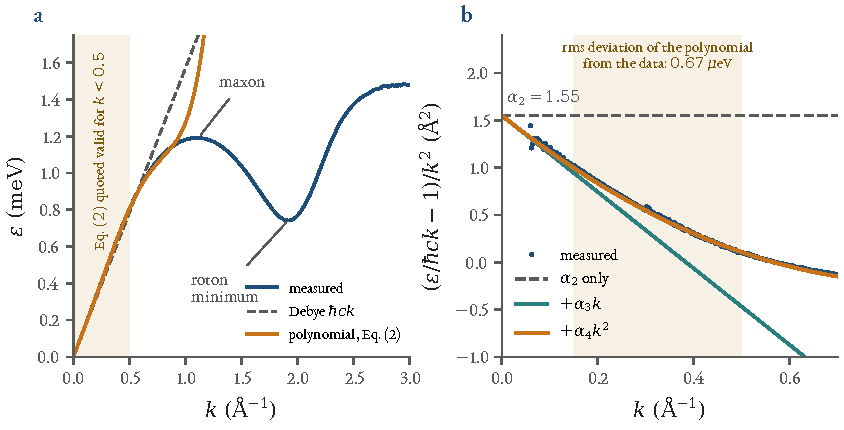
\includegraphics[width=\linewidth]{figures/ch04_dispersion.pdf}
\caption[The phonon branch of superfluid helium-4 measured by neutron scattering]{The phonon branch of superfluid $^4$He at saturated vapour pressure ($T<0.1\cfK$), measured by neutron scattering (ancillary data of \cite{Godfrin2021}, CC BY 4.0). \textbf{(a)} The measured curve (blue), the linear Debye dispersion (dashed grey) and the polynomial of Eq.~(2) of the paper with the coefficient set quoted there (orange); maxon at $k=\cfv{maxon-k}\ \cfAng^{-1}$, roton minimum at $k=\cfv{roton-k}\ \cfAng^{-1}$, $\varepsilon/\cfkB=\cfv{roton-K}\cfK$ in this table. \textbf{(b)} The same data divided by $\hbar ck$ and $k^2$: the intercept is $\alpha_2$, the slope $\alpha_3$, the curvature $\alpha_4$. The rms difference between the polynomial and the table for $0.15\le k\le0.5\ \cfAng^{-1}$ is $\cfv{rms-ueV}\ \mu$eV.}\label{ch04:fig-dispersion}
\end{figure}

Real helium is not linear.
The paper writes the phonon branch as a power series
\begin{equation}\label{ch04:eq-disp}
 \varepsilon(k)=\hbar c\,k\,\bigl(1+\alpha_2k^2+\alpha_3k^3+\alpha_4k^4+\alpha_5k^5+\alpha_6k^6\bigr),
\end{equation}
with no linear term in the bracket ($\alpha_1=0$); $\alpha_j$ has the dimension of length$^j$.
For saturated vapour pressure it quotes $c=\cfv{c}\ \mathrm{m\,s^{-1}}$, $\alpha_2=\cfv{a2}\ \cfAng^2$, $\alpha_3=\cfv{a3}\ \cfAng^3$, $\alpha_4=\cfv{a4}\ \cfAng^4$ and $\alpha_5=\alpha_6=0$, and says that this set describes the measured dispersion for $k<0.5\ \cfAng^{-1}$.
\Cref{ch04:fig-dispersion} compares it with the open table: within the shaded range the polynomial and the data differ by $\cfv{rms-ueV}\ \mu$eV rms and by at most $\cfv{maxdev-ueV}\ \mu$eV, and at $k=1\ \cfAng^{-1}$ the polynomial lies $\cfv{poly-dev-1}$ per cent above the data: beyond its range it stops describing helium and becomes a sequence of numbers (that is not a criticism, the range is quoted with the coefficients; it is the first hint of what a series in $T$ can and cannot do).

The sign of $\alpha_2$ matters physically.
For $\alpha_2>0$ the energy at a given $k$ lies above the linear Debye value, so there are fewer thermal phonons than in a Debye gas and $C_V/T^3$ \emph{falls} as the temperature rises: this is the slow drift of the first paragraph.
(The same sign, the ``anomalous'' dispersion, keeps the collinear decay of a phonon into two phonons energetically open: this is \Lthm{HeliumKinematics}{three_phonon_open_iff}, for a dispersion $ck(1+ak^2)$; \cref{ch05} treats it.)

\subsection{A series in \texorpdfstring{$T$}{T}}
To turn \eqref{ch04:eq-energy} into a series one needs the integral over energy, not over wavevector.
Write $u=\varepsilon/\hbar c$, which has the dimension of an inverse length, so that $u=k(1+\alpha_2k^2+\dots)$, and invert the series:
\begin{equation}\label{ch04:eq-inverse}
 k(u)=u-\alpha_2u^3-\alpha_3u^4+(3\alpha_2^2-\alpha_4)u^5+(7\alpha_2\alpha_3-\alpha_5)u^6+\eta\,u^7+O(u^8),
\end{equation}
with $\eta=-12\alpha_2^3+8\alpha_2\alpha_4+4\alpha_3^2-\alpha_6$.
This is the inverse series printed in the paper, here for $\alpha_1=0$ (the paper prints it for general $\alpha_1$).
The density of states in $u$ is $k^2\,\mathrm dk/\mathrm du=\sum_n g_n u^n$ with
\begin{equation}\label{ch04:eq-dos}
\begin{aligned}
 g_2&=1,\quad g_3=0,\quad g_4=-5\alpha_2,\quad g_5=-6\alpha_3,\quad g_6=7(4\alpha_2^2-\alpha_4),\\
 g_7&=8(9\alpha_2\alpha_3-\alpha_5),\quad g_8=-3(55\alpha_2^3-30\alpha_2\alpha_4-15\alpha_3^2+3\alpha_6).
\end{aligned}
\end{equation}
Each monomial $g_nu^n$ gives a thermal integral that is a Bose integral,
\begin{equation}\label{ch04:eq-bose}
 \int_0^\infty\frac{u^{m}}{e^{\hbar cu/\cfkB T}-1}\,\mathrm du=\Bigl(\frac{\cfkB T}{\hbar c}\Bigr)^{m+1}\,m!\,\zeta(m+1),
\end{equation}
so that
\begin{align}
 E(T)&=\frac{V}{2\pi^2}\sum_n g_n\,(n+1)!\,\zeta(n+2)\,\frac{(\cfkB T)^{n+2}}{(\hbar c)^{n+1}},\label{ch04:eq-series-E}\\
 C_V&=\sum_n\frac{V\cfkB^{\,n+2}}{2\pi^2(\hbar c)^{n+1}}\,g_n\,(n+2)!\,\zeta(n+2)\;T^{\,n+1}.\label{ch04:eq-series}
\end{align}
The term $n=2$ is Debye's.
The term $n=3$ would give a $T^4$ term, but $g_3=0$ because there is no $\alpha_1$: that is why Eq.~(22) has no $B\,T^4$.
The terms $n=4,5,6,7,8$ give $C\,T^5$, $D\,T^6$, $E\,T^7$, $K\,T^8$, $L\,T^9$, and the result is \cref{ch04:tab-coeffs}.

\begin{table}[t]\centering\small
\caption{The six coefficients of Eq.~(22). Column $g_n$: bracket of the density of states \eqref{ch04:eq-dos}; column $I_n$: the Bose integral $\int_0^\infty t^{n+1}/(e^t-1)\,\mathrm dt=(n+1)!\,\zeta(n+2)$ (all six values are proved in Lean, Section~\ref{ch04:sec-lean}); last two columns: the closed form evaluated with the coefficient set of the paper (units $\mathrm{J\,mol^{-1}K^{-p}}$, $p$ the power of $T$; values from \texttt{figures/ch04\_common.py}), and the number printed in the paper.}\label{ch04:tab-coeffs}
\renewcommand{\arraystretch}{1.25}
\begin{tabular}{@{}llllrr@{}}\toprule
 & $T^p$ & $g_n$ & $I_n$ & computed & printed \\ \midrule
 $A$ & $T^3$ & $1$ & $\pi^4/15$ & \cfv{A-val} & \cfv{A-pr} \\
 $C$ & $T^5$ & $-5\alpha_2$ & $8\pi^6/63$ & \cfv{C-val} & \cfv{C-pr} \\
 $D$ & $T^6$ & $-6\alpha_3$ & $720\,\zeta(7)$ & \cfv{D-val} & \cfv{D-pr} \\
 $E$ & $T^7$ & $7(4\alpha_2^2-\alpha_4)$ & $8\pi^8/15$ & \cfv{E-val} & \cfv{E-pr} \\
 $K$ & $T^8$ & $8(9\alpha_2\alpha_3-\alpha_5)$ & $40320\,\zeta(9)$ & \cfv{K-val} & \cfv{K-pr} \\
 $L$ & $T^9$ & $-3(55\alpha_2^3-30\alpha_2\alpha_4-15\alpha_3^2+3\alpha_6)$ & $128\pi^{10}/33$ & \cfv{L-val} & \cfv{L-pr} \\ \bottomrule
\end{tabular}
\end{table}

Written out, with $\zeta$ the Riemann zeta function, the six coefficients are
\begin{align*}
 A&=\frac{2\pi^2\cfkB^4V}{15\,c^3\hbar^3}, &
 C&=-\frac{40\,\pi^4\alpha_2\cfkB^6V}{21\,c^5\hbar^5},\\
 D&=-\frac{15120\,\alpha_3\cfkB^7V\,\zeta(7)}{\pi^2c^6\hbar^6}, &
 E&=\frac{224\,\pi^6\cfkB^8V\,(4\alpha_2^2-\alpha_4)}{15\,c^7\hbar^7},\\
 K&=\frac{1451520\,\cfkB^9V\,\zeta(9)\,(9\alpha_2\alpha_3-\alpha_5)}{\pi^2c^8\hbar^8},\\
 L&=-\frac{640\,\pi^8\cfkB^{10}V\,(55\alpha_2^3-30\alpha_2\alpha_4-15\alpha_3^2+3\alpha_6)}{11\,c^9\hbar^9}.
\end{align*}
Three features are structural, not matters of presentation.
First, $\pi$ appears in $A,C,E,L$ and $\zeta(7)$, $\zeta(9)$ in $D$ and $K$: even zeta values at $2k$ are rational multiples of $\pi^{2k}$ (Bernoulli numbers), odd ones are not known in closed form, and \eqref{ch04:eq-series} contains $\zeta(n+2)$, which is even for $n$ even and odd for $n$ odd.
Second, the coefficients are not one-to-one with the $\alpha_j$: $E$ contains $\alpha_2$ and $\alpha_4$, $L$ contains $\alpha_2$, $\alpha_3$, $\alpha_4$ and $\alpha_6$, so a measurement of $E$ gives a combination of dispersion coefficients, not $\alpha_4$.
Third, the printed numbers of \cref{ch04:tab-coeffs} follow from the printed formulas at the quoted coefficients to within $\cfv{coef-maxdiff}$ per cent (the quoted $\alpha_j$ are themselves rounded, so a few parts in $10^3$ carry no information).
That is a check of the paper's arithmetic; it is not yet a check of its formulas, which is where an error of an earlier series would have lived.


%% ====================================================================================================================
\section{What the proof assistant says}\label{ch04:sec-lean}

The library \texttt{QuantumFluids} has three modules for this chapter, \texttt{BoseIntegral}, \texttt{PhononSeries} and \texttt{PhononSpecificHeat}, with a design note recording how the work was done (the file \texttt{PHONON\_SERIES\_A\_TO\_L.md} in the \texttt{docs/designs} directory of the repository).
\Cref{ch02} explains how to read Lean; here it is enough to know that a \texttt{theorem} is a statement together with a proof that the kernel has checked, and that the statements below are copied from the library unchanged.
For this book the three modules were compiled, in dependency order, with Lean \cfv{lean-toolchain} against the library's Mathlib: no errors, no \texttt{sorry}.
The only axioms used are the three of classical mathematics (\texttt{propext}, \texttt{Classical.choice}, \texttt{Quot.sound}) for \texttt{BoseIntegral} and \texttt{PhononSpecificHeat}, and just \texttt{propext} and \texttt{Quot.sound} for \texttt{PhononSeries}, which is pure ring theory.

\subsection{Step one: the Bose integral}
Every coefficient of Eq.~(22) rests on one identity, $\int_0^\infty t^n/(e^t-1)\,\mathrm dt=n!\,\zeta(n+1)$.
Mathlib has the Gamma integral and $\zeta(2k)$ in closed form, but not this integral, so the library proves it.

\begin{leanbox}{BoseIntegral}
\begin{lstlisting}[style=lean,basicstyle=\ttfamily\footnotesize]
/-- The Bose factor `1/(eᵗ − 1)`, complex-valued so that Mathlib's `mellin` applies. -/
noncomputable def bose (t : ℝ) : ℂ := ((1 / (rexp t - 1) : ℝ) : ℂ)

theorem bose_integral_nat {n : ℕ} (hn : 1 ≤ n) :
    mellin bose (n + 1) = (Nat.factorial n : ℂ) * riemannZeta (n + 1)
-- statement only; the proof is in lean_src/BoseIntegral.lean
\end{lstlisting}
\end{leanbox}

\noindent In words.
Mathlib's \lean{mellin f s} is by definition $\int_0^\infty t^{s-1}f(t)\,\mathrm dt$, so \lean{mellin bose (n + 1)} \emph{is} the integral $\int_0^\infty t^n/(e^t-1)\,\mathrm dt$.
The first theorem, \Lthm{BoseIntegral}{bose_integral_nat}, says it equals $n!\,\zeta(n+1)$ for every $n\ge1$: this is \eqref{ch04:eq-bose} with the temperature scaled out.
A companion theorem, \Lthm{BoseIntegral}{debye_specific_heat}, says that the energy $\pi^2V(\cfkB T)^4/30(\hbar c)^3$ of the Debye gas, whose integral is the case $n=3$ (\Lthm{BoseIntegral}{mellin_bose_four}: \lean{mellin bose 4} $=\pi^4/15$), has the derivative $A\,T^3$ with $A=2\pi^2\cfkB^4V/15c^3\hbar^3$, the coefficient printed in the paper.
\emph{Proof idea (abridged).} For $t>0$ one has $1/(e^t-1)=\sum_{m\ge0}e^{-(m+1)t}$, the geometric series behind Bose statistics (\Lthm{BoseIntegral}{hasSum_bose}); Mathlib's \lean{hasSum\_mellin} integrates a series of exponentials term by term, each term giving $\Gamma(s)/(m+1)^s$; the sum is $\Gamma(s)\zeta(s)$, and $\Gamma(n+1)=n!$.

\subsection{Step two: inverting the dispersion and counting states, without analysis}
The next module is where the printed series meet algebra.
The claim ``$k(u)$ is the inverse series up to $O(u^8)$'' involves a truncation, and a truncation normally brings questions of convergence with it.
The library avoids them.
\emph{Equal up to $O(e^8)$} is stated as an identity in an arbitrary commutative ring $R$ with an element $e$ such that $e^8=0$.
Taking $R$ to be the ring of power series modulo $e^8$ recovers the usual statement; nothing about limits is needed, and the theorem is pure ring theory.

\begin{leanbox}{PhononSeries}
\begin{lstlisting}[style=lean,basicstyle=\ttfamily\footnotesize]
variable {R : Type*} [CommRing R]

/-- The inverse series for `alpha_1 = 0`, the case the paper's Eq. (22) treats. -/
def kInv0 (a2 a3 a4 a5 a6 e : R) : R :=
  -12*a2^3*e^7 + 3*a2^2*e^5 + 7*a2*a3*e^6 + 8*a2*a4*e^7 - a2*e^3 + 4*a3^2*e^7 - a3*e^4 - a4*e^5 - a5*e^6 - a6*e^7 + e

/-- Its formal derivative with respect to `e`. -/
def kInv0Deriv (a2 a3 a4 a5 a6 e : R) : R :=
  -84*a2^3*e^6 + 15*a2^2*e^4 + 42*a2*a3*e^5 + 56*a2*a4*e^6 - 3*a2*e^2 + 28*a3^2*e^6 - 4*a3*e^3 - 5*a4*e^4 - 6*a5*e^5 - 7*a6*e^6 + 1

theorem density_of_states (a2 a3 a4 a5 a6 e : R) (h : e ^ 9 = 0) :
    kInv0 a2 a3 a4 a5 a6 e ^ 2 * kInv0Deriv a2 a3 a4 a5 a6 e
      = e ^ 2 - 5 * a2 * e ^ 4 - 6 * a3 * e ^ 5 + 7 * (4 * a2 ^ 2 - a4) * e ^ 6
        + 8 * (9 * a2 * a3 - a5) * e ^ 7
        - 3 * (55 * a2 ^ 3 - 30 * a2 * a4 - 15 * a3 ^ 2 + 3 * a6) * e ^ 8
-- statement only; the proof is in lean_src/PhononSeries.lean
\end{lstlisting}
\end{leanbox}

\noindent In words.
The module proves two theorems.
The first, \Lthm{PhononSeries}{dispersion_kInv}, says that the inverse series printed in the paper, for general $\alpha_1$ and through $(\omega/c)^7$ with the coefficient $\eta$, really inverts $u=k(1+\alpha_1k+\dots+\alpha_6k^6)$: substitute it in and you get $e$ back, modulo $e^8$ (it is stated for the series \lean{kInv} of general $\alpha_1$, of which \lean{kInv0} is the case $\alpha_1=0$).
The second, shown above, \Lthm{PhononSeries}{density_of_states}, says that $k^2\,\mathrm dk/\mathrm du$, computed from the series \eqref{ch04:eq-inverse} for $\alpha_1=0$ and its derivative, equals the polynomial whose coefficients are the brackets \eqref{ch04:eq-dos}, modulo $e^9$.
The missing term $e^3$ is the missing $B\,T^4$.
\emph{Proof idea (abridged).} The powers $k^2,\dots,k^7$ of the series are truncated one at a time, each step a statement of the form \lean{linear\_combination (r) * h} with $h:\ e^8=0$.
This tactic asks the kernel to check that (left side $-$ right side) $-\,r\cdot e^N$ vanishes identically as a polynomial ($N=8$ or $9$); $r$ is the \emph{certificate}.
Here is the shape of one such proof, with its certificate shortened:
\begin{lstlisting}[style=lean,basicstyle=\ttfamily\footnotesize]
theorem kSq0_eq (a2 a3 a4 a5 a6 e : R) (h : e ^ 9 = 0) :
    kInv0 a2 a3 a4 a5 a6 e ^ 2 = kSq0 a2 a3 a4 a5 a6 e := by
  unfold kInv0 kSq0
  linear_combination (144*a2^6*e^5 - 72*a2^5*e^3 - 168*a2^4*a3*e^4 - 192*a2^4*a4*e^5 + ...) * h
\end{lstlisting}
\noindent (proof abridged: the certificate has \cfv{cert-kSq0} terms; the six certificates for the powers $k^2,\dots,k^7$ of the general inverse series have \cfv{cert-list} terms.)
The certificates were produced by a computer-algebra script and are \emph{checked, not trusted}: had the script made an error the kernel would reject the proof.
The design note records this module as the first generated proof file in the library.

\subsection{Step three: the six coefficients}
The last module assembles the two ingredients.
The energy carried by the monomial $g\,u^n$ of the density of states is, from \eqref{ch04:eq-series-E}, $\frac{V}{2\pi^2}\,g\,I\,\cfkB^{n+2}T^{n+2}/(\hbar c)^{n+1}$ with $I=\int_0^\infty t^{n+1}/(e^t-1)\,\mathrm dt$ the Bose integral.
The library calls it \Lthm{PhononSpecificHeat}{energyTerm}.

\begin{leanbox}{PhononSpecificHeat}
\begin{lstlisting}[style=lean,basicstyle=\ttfamily\footnotesize]
noncomputable def energyTerm (V kB hbar c g : ℝ) (n : ℕ) (I T : ℝ) : ℝ :=
  V / (2 * π ^ 2) * g * I * kB ^ (n + 2) / (hbar * c) ^ (n + 1) * T ^ (n + 2)

theorem phonon_specific_heat (V kB hbar c a2 a3 a4 a5 a6 z7 z9 T : ℝ) (hh : hbar ≠ 0) (hc : c ≠ 0) :
    HasDerivAt (fun T =>
        energyTerm V kB hbar c 1 2 (π ^ 4 / 15) T
      + energyTerm V kB hbar c (-5 * a2) 4 (8 * π ^ 6 / 63) T
      + energyTerm V kB hbar c (-6 * a3) 5 (720 * z7) T
      + energyTerm V kB hbar c (7 * (4 * a2 ^ 2 - a4)) 6 (8 * π ^ 8 / 15) T
      + energyTerm V kB hbar c (8 * (9 * a2 * a3 - a5)) 7 (40320 * z9) T
      + energyTerm V kB hbar c (-3 * (55 * a2 ^ 3 - 30 * a2 * a4 - 15 * a3 ^ 2 + 3 * a6)) 8
          (128 * π ^ 10 / 33) T)
      ( 2 * π ^ 2 * kB ^ 4 * V / (15 * c ^ 3 * hbar ^ 3) * T ^ 3
      + -(40 * (π ^ 4 * a2 * kB ^ 6 * V)) / (21 * (c ^ 5 * hbar ^ 5)) * T ^ 5
      + -(15120 * (a3 * kB ^ 7 * V * z7)) / (π ^ 2 * c ^ 6 * hbar ^ 6) * T ^ 6
      + 224 * π ^ 6 * kB ^ 8 * V * (4 * a2 ^ 2 - a4) / (15 * c ^ 7 * hbar ^ 7) * T ^ 7
      + 1451520 * kB ^ 9 * V * z9 * (9 * a2 * a3 - a5) / (π ^ 2 * c ^ 8 * hbar ^ 8) * T ^ 8
      + -(640 * (π ^ 8 * kB ^ 10 * V * (55 * a2 ^ 3 - 30 * a2 * a4 - 15 * a3 ^ 2 + 3 * a6)))
          / (11 * (c ^ 9 * hbar ^ 9)) * T ^ 9) T
-- statement only; the proof is in lean_src/PhononSpecificHeat.lean
\end{lstlisting}
\end{leanbox}

\noindent In words.
A theorem proved earlier in the module, \Lthm{PhononSpecificHeat}{bose_integral_values}, gives the six Bose integrals of \cref{ch04:tab-coeffs} in closed form: $\int_0^\infty t^3/(e^t-1)\,\mathrm dt=\pi^4/15$, then $8\pi^6/63$, $720\,\zeta(7)$, $8\pi^8/15$, $40320\,\zeta(9)$, $128\pi^{10}/33$ (as \lean{mellin bose 4}, $\dots$, \lean{mellin bose 10}).
The even ones use Mathlib's $\zeta(2k)$ through Bernoulli numbers (the library computes $B_6=\tfrac1{42}$, $B_8=-\tfrac1{30}$, $B_{10}=\tfrac5{66}$, because Mathlib's table stops at $B_4$, and from them $\zeta(6)=\pi^6/945$, $\zeta(8)=\pi^8/9450$, $\zeta(10)=\pi^{10}/93555$); the odd ones stay symbolic.
The capstone \Lthm{PhononSpecificHeat}{phonon_specific_heat} says: \emph{the derivative with respect to $T$ of the sum of the six energy terms --- with the density-of-states brackets of \lean{density\_of\_states} and the six Bose integrals --- is exactly the six printed closed forms $A,C,D,E,K,L$}.
The two odd zeta values enter as real parameters \lean{z7}, \lean{z9}; \lean{bose\_integral\_values} is where they are tied to \lean{riemannZeta 7} and \lean{riemannZeta 9}, which keeps the capstone in $\mathbb R$ and makes the absence of a closed form visible in the type.
\emph{Proof idea (abridged).} Each term differentiates by the power rule; \lean{HasDerivAt.add} is applied five times; the two sides then differ only by rearrangement, which \lean{field\_simp} and \lean{ring} close.

\subsection{Closing the links that were made by inspection}\label{ch04:sec-newlean}
Reading the three boxes again, one sees what the design note itself records as the weak points: the chain from the dispersion to Eq.~(22) is assembled by \emph{retyping}.
The brackets $1,-5\alpha_2,-6\alpha_3,\dots$ in the capstone were copied from \lean{density\_of\_states}; no theorem says that they are the coefficients of the polynomial \lean{kInv0}$^2\cdot$\lean{kInv0Deriv}.
\lean{kInv0Deriv} was typed in, not computed as a derivative.
And the six values of $I$ in the capstone were retyped from \lean{bose\_integral\_values}.
None of these is likely to hide an error, but it is exactly the kind of gap that a ``machine-checked'' label can paper over.


The file \texttt{lean/Ch04\_DosLink.lean} of this book removes the retypings.
It is \emph{new Lean, written for this book and not part of the library}: it imports the three modules above, lives in the namespace \texttt{QuantumFluids.DosLink}, and compiles in about a minute against the same Mathlib, with no error and no \lean{sorry}; its \lean{\#print axioms} lines show the three axioms of classical mathematics and nothing else.

\begin{leanbox}{new: Ch04\_DosLink}
\begin{lstlisting}[style=lean,basicstyle=\ttfamily\footnotesize]
/-- The inverse series with the dispersion coefficients as constant polynomials, evaluated at `X`. -/
noncomputable def kPoly (a2 a3 a4 a5 a6 : ℝ) : ℝ[X] :=
  kInv0 (C a2) (C a3) (C a4) (C a5) (C a6) X

theorem derivative_kPoly (a2 a3 a4 a5 a6 : ℝ) :
    derivative (kPoly a2 a3 a4 a5 a6) = kInv0Deriv (C a2) (C a3) (C a4) (C a5) (C a6) X

/-- The density-of-states polynomial `k(e)^2 * dk/de`, with `dk/de` the formal derivative. -/
noncomputable def dosPoly (a2 a3 a4 a5 a6 : ℝ) : ℝ[X] :=
  kPoly a2 a3 a4 a5 a6 ^ 2 * derivative (kPoly a2 a3 a4 a5 a6)

theorem dos_coeffs (a2 a3 a4 a5 a6 : ℝ) :
    (dosPoly a2 a3 a4 a5 a6).coeff 2 = 1 ∧
    (dosPoly a2 a3 a4 a5 a6).coeff 3 = 0 ∧
    (dosPoly a2 a3 a4 a5 a6).coeff 4 = -5 * a2 ∧
    (dosPoly a2 a3 a4 a5 a6).coeff 5 = -6 * a3 ∧
    (dosPoly a2 a3 a4 a5 a6).coeff 6 = 7 * (4 * a2 ^ 2 - a4) ∧
    (dosPoly a2 a3 a4 a5 a6).coeff 7 = 8 * (9 * a2 * a3 - a5) ∧
    (dosPoly a2 a3 a4 a5 a6).coeff 8 = -3 * (55 * a2 ^ 3 - 30 * a2 * a4 - 15 * a3 ^ 2 + 3 * a6)
\end{lstlisting}
\begin{lstlisting}[style=lean,basicstyle=\ttfamily\fontsize{7.2}{8.6}\selectfont]
theorem phonon_specific_heat_end_to_end (V kB hbar c a2 a3 a4 a5 a6 T : ℝ) (hh : hbar ≠ 0) (hc0 : c ≠ 0) :
    HasDerivAt (fun T =>
        energyTerm V kB hbar c ((dosPoly a2 a3 a4 a5 a6).coeff 2) 2 (mellin bose 4).re T
      + energyTerm V kB hbar c ((dosPoly a2 a3 a4 a5 a6).coeff 4) 4 (mellin bose 6).re T
      + energyTerm V kB hbar c ((dosPoly a2 a3 a4 a5 a6).coeff 5) 5 (mellin bose 7).re T
      + energyTerm V kB hbar c ((dosPoly a2 a3 a4 a5 a6).coeff 6) 6 (mellin bose 8).re T
      + energyTerm V kB hbar c ((dosPoly a2 a3 a4 a5 a6).coeff 7) 7 (mellin bose 9).re T
      + energyTerm V kB hbar c ((dosPoly a2 a3 a4 a5 a6).coeff 8) 8 (mellin bose 10).re T)
      (…) T      -- abridged: the six closed forms of `phonon_specific_heat`, not repeated
-- statements only; the proofs are in lean/Ch04_DosLink.lean
\end{lstlisting}
\end{leanbox}

\noindent In words.
\Lthm{DosLink}{kPoly} is the inverse series \lean{kInv0} with the dispersion coefficients as constant polynomials, evaluated at the variable $X$ of $\mathbb R[X]$; \Lthm{DosLink}{derivative_kPoly} says that Mathlib's formal derivative of it \emph{is} \lean{kInv0Deriv}, which is thus no longer typed in.
\Lthm{DosLink}{dosPoly} is $k^2\cdot k'$ as an honest polynomial, and \Lthm{DosLink}{dos_coeffs} says that its coefficients in degrees $2$ to $8$ are exactly the brackets \eqref{ch04:eq-dos}, the absent degree~$3$ included.
\Lthm{DosLink}{phonon_specific_heat_end_to_end} is Eq.~(22) with nothing retyped: the brackets are read off \lean{dosPoly}, the six Bose integrals are the real parts of \lean{mellin bose 4}, \dots, \lean{mellin bose 10}, and the two odd zeta values are $\zeta(7)$ and $\zeta(9)$ themselves.

\emph{Proof idea (abridged).} Apply \Lthm{PhononSeries}{density_of_states} not in $\mathbb R$ but in the ring $\mathbb R[X]/(X^9)$, where $e=X$ satisfies $e^9=0$.
It says that $k^2k'$ and the polynomial of brackets are equal there, that is, that $X^9$ divides their difference, and a polynomial divisible by $X^9$ has vanishing coefficients below degree $9$ (\lean{Polynomial.X\_pow\_dvd\_iff}).
The end-to-end theorem then follows from \Lthm{PhononSpecificHeat}{phonon_specific_heat} and \Lthm{PhononSpecificHeat}{bose_integral_values}.

The file goes one step further.
It defines the energy of the monomial $g\,u^n$ as the integral itself, written with Mathlib's Mellin transform (\lean{energyMonomial}); proves, in \Lthm{DosLink}{energyMonomial_eq}, that for $T>0$ it equals \lean{energyTerm} evaluated with the Bose integral $\operatorname{Re}\,\lean{mellin bose (n + 2)}$; and restates Eq.~(22), in \Lthm{DosLink}{phonon_specific_heat_integral}, for the sum of the six integrals.


\paragraph{What is still outside Lean.}
What these theorems say is exact and limited: the derivative of the thermal energy of the \emph{truncated} density of states $\sum_{n=2}^{8}g_nu^n$, integrated against the Bose factor over $(0,\infty)$, is Eq.~(22).
That the truncated sum may stand for the true density of states under the integral --- that the series is an asymptotic expansion of the specific heat of a given dispersion curve, with the roton branch and the upper limit dropped --- is an analytical statement that the library does not contain.
Section~\ref{ch04:sec-data} computes what it amounts to.



%% ====================================================================================================================
\section{A confirmation, not a finding}\label{ch04:sec-confirm}

Lean is one derivation.
Two others were made without it, for the reason that two thermometers matter: a proof assistant checks a \emph{statement}, so it can confirm a derivation that started from the wrong statement just as faithfully as from the right one.

\paragraph{A symbolic derivation.}
The script \texttt{exploration/godfrin/derive\_cv\_series.py} derives everything from scratch with the computer-algebra system sympy: it reverts the series order by order, forms $\mathrm d(k^3/3)/\mathrm du$, integrates term by term with the Bose integral \eqref{ch04:eq-bose}, differentiates, and compares each result with the printed closed form by the exact test \lean{simplify(derived - printed) == 0}, which leaves no room for tuning.
I re-ran it for this book (\cfv{sympy-seconds} s on the shared machine); its output ends:
\begin{lstlisting}[style=plainmono,basicstyle=\ttfamily\footnotesize]
A (T^3): MATCHES the printed closed form      C (T^5): MATCHES the printed closed form
D (T^6): MATCHES the printed closed form      E (T^7): MATCHES the printed closed form
K (T^8): MATCHES the printed closed form      L (T^9): MATCHES the printed closed form
T^4 coefficient (paper: absent because alpha_1 = 0): 0
INVERSE SERIES: all 7 printed coefficients match
C_V SERIES: ALL SIX MATCH
\end{lstlisting}
(``All 7'' counts the seven coefficients of the printed inverse series for general $\alpha_1$, through $(\omega/c)^7$.)

\paragraph{Exact rational arithmetic.}
The third derivation is this chapter's own, written to be as unlike the other two as possible: no symbols, no proof, only fractions.
With the coefficient set of the paper as the exact fractions $\alpha_2=31/20$, $\alpha_3=-101/25$, $\alpha_4=23/10$, the script \texttt{figures/ch04\_series\_ext.py} reverts the series by fixed-point iteration in Python's \texttt{fractions} and reads off the density-of-states coefficients, $g_4=-31/4$, $g_5=606/25$, $g_6=5117/100$, $g_7=-56358/125$, $g_8=3527061/8000$: the brackets \eqref{ch04:eq-dos} at those $\alpha$'s, obtained by a program that has never seen them.
Multiplying by the Bose integrals gives the coefficient of each power of $T$; the six that Eq.~(22) predicts agree with the closed forms to a relative \cfv{rat-maxdiff} (double-precision rounding), and the coefficient of $T^4$ is exactly zero.
The same script continues past $L$, giving $c_{10}=\cfv{c10}$ and $c_{11}=\cfv{c11}$ (in $\mathrm{J\,mol^{-1}K^{-p}}$): Lean does not cover those, the exact arithmetic does, and Section~\ref{ch04:sec-data} uses them.

\paragraph{What kind of check this is.}
An earlier pass in the programme had only reproduced the six printed \emph{numbers} from the six printed \emph{formulas} (the last column of \cref{ch04:tab-coeffs}).
That tests the arithmetic of the paper, not its formulas, and a formula is where an error of an earlier series would live.
The programme's rule LL-15 (name the property a claim depends on, and check that property rather than a neighbour of it) asks for a derivation from the dispersion relation, and that is what the three above are.
They agree with Eq.~(22) in all six coefficients, with the inverse series, and with the absence of a $T^4$ term.

\paragraph{Checkers must be able to fail.}
A proof checker that cannot reject anything proves nothing.
When the Lean proofs were first written, four deliberately wrong versions were fed to it --- $-12\alpha_2^3$ in $\eta$ changed to $-11\alpha_2^3$, the $15120$ of $D$ to $15121$, the $9\alpha_2\alpha_3$ of $K$ to $8\alpha_2\alpha_3$, the $55$ of $L$ to $54$ --- and all four were rejected (design note).
I repeated two of them for this book, against the library modules compiled as above (the files \texttt{lean/Ch04\_NegativeControl\_L54.lean} and \texttt{lean/Ch04\_NegativeControl\_D15121.lean} are meant to fail; paths shortened in what follows, and the dagger that Lean prints after inaccessible names removed).
Changing $55$ to $54$ in \Lthm{PhononSeries}{density_of_states}, with the certificate of the true theorem, gives:
\lstinputlisting[style=plainmono,basicstyle=\ttfamily\footnotesize]{figures/ch04_negctl_L54.txt}
\noindent and changing the $15120$ of $D$ to $15121$ in the capstone \Lthm{PhononSpecificHeat}{phonon_specific_heat} gives:
\lstinputlisting[style=plainmono,basicstyle=\ttfamily\footnotesize]{figures/ch04_negctl_D15121.txt}
\noindent In the first case \lean{ring} prints the residue: the two sides differ by $-3a_2^3e^8$, exactly what changing $55$ to $54$ in the term $-3(55a_2^3-\dots)e^8$ must leave behind.
In the second the message is a polynomial identity that \lean{ring} could not close, too long to show; what matters is that it was not closed.
A proof that fails, with a residue one can read, is a checker doing its work.

\paragraph{The outcome rule, and a lapse.}
The programme's discipline is to fix, before running a check, what each outcome will be called.
Here that was \emph{not} done: the derivation script was written and run first and the rule below afterwards, and the design note records a process lapse.
Because the comparison is a symbolic identity, with no tolerance to tune and no analysis choice (the coefficients to compare are the paper's own), the lapse cannot have shaped the result; it is recorded all the same.
The rule that binds what follows: a mismatch would have been a candidate misprint of the preprint, to be settled against the published version before anything is said about the paper; a full match is a confirmation, and \emph{is not to be dressed up as a finding}.
It was a full match, for the arXiv version; the version of record was not compared.
Eq.~(22) is a correct consequence of Eq.~(2), as a statement of mathematics.
That is a good thing to know about a series whose predecessors were wrong, and it is all it is.


%% ====================================================================================================================
\section{What the solver says}\label{ch04:sec-solver}

The solver is a witness for a different question.
Lean says that, for the polynomial dispersion \eqref{ch04:eq-disp}, the coefficients of the series in $T$ are what Eq.~(22) says.
A solver that has never heard of a series can be asked whether the \emph{integral itself} behaves as that series says.
Two experiments follow.
Neither is a proof: each carries a tolerance below which it is blind, and each concerns the model polynomial and not helium.
All integrals use CVODE of rusty-SUNDIALS through its Python module (\texttt{rusty\_sundials.CvodeSolver}), with the Adams--Moulton option, the natural one for smooth non-stiff problems.

\paragraph{Which build of the solver.}
My first runs used the module installed in the project's virtual environment (built 2026-09-26) and gave plausible numbers that were wrong: at relative tolerance $10^{-6}$ its Adams method returned the Debye integral $\int_0^{70}x^3/(e^x-1)\,\mathrm dx$ with a relative error $\cfv{old-adams-bose-err}$ after $\cfv{old-adams-bose-calls}$ right-hand-side calls, $\cfv{old-adams-bose-ratio}$ times the tolerance, and its BDF gave up (``too many error test failures at one step'') on \cfv{old-bdf-landing-err} of \cfv{probe-landing-n} end points when asked for the six Bose integrals of the next subsection (\texttt{figures/ch04\_solver\_probe.py}).
The maintainers' note \texttt{docs/CVODE\_ADAMS\_FIX.md} in the rusty-SUNDIALS repository describes the cause: in that build \lean{Method::Adams} was implicit Euler with a Milne error estimate, a first-order method whose error scales like $\sqrt{\mathrm{rtol}}$, as observed; it was fixed on 2026-09-28.
Every number of this chapter comes from a build of rusty-SUNDIALS commit \cfv{rs-commit-short} (sha256 of \texttt{rusty\_sundials.so} beginning \cfv{rs-sha-short}), and the scripts refuse to run with any other: Adams on $y'=-y$ over $[0,10]$ at relative tolerance $10^{-8}$ must use fewer than $5000$ right-hand-side calls (it uses \cfv{new-adams-decay-calls}).
With that build the Debye integral costs $\cfv{new-adams-bose-calls}$ calls at relative tolerance $10^{-6}$ and returns a relative error $\cfv{new-adams-bose-err}$, and no end point defeats Adams or BDF (\cfv{new-landing-err} give-ups).
A numerical result with the right shape is not evidence that the tool is right; a check against a closed form is.

\subsection{The Bose integrals as initial-value problems}
The integral $\int_0^X t^m/(e^t-1)\,\mathrm dt$ is the value at $x=X$ of the solution of $y'=x^m/(e^x-1)$, $y(0)=0$.
Scaling by $m!$ makes all six components of order one ($y_m\to\zeta(m+1)$), which lets one scalar absolute tolerance serve all of them.
The comparison is with the closed forms \emph{proved in Lean} (\cref{ch04:tab-coeffs}), not with a numerically evaluated $m!\,\zeta(m+1)$.

\begin{rustbox}{CVODE: the six Bose integrals}
\begin{lstlisting}[style=py,basicstyle=\ttfamily\footnotesize]
def rhs_bose(x, y):                    # y_m' = x^m / (m! (e^x - 1)),  y_m(0) = 0
    if x <= 0.0:
        return [0.0]*len(ms)
    e = np.expm1(x)
    return [x**m/(fact[m]*e) for m in ms]
# ms = [3, 5, 6, 7, 8, 9];  excerpt of figures/ch04_cvode_compute.py
solver = rs.CvodeSolver("adams", rtol, atol, 200_000)    # method, rtol, atol, max_steps
_, y = solver.solve(rhs_bose, 0.0, [0.0]*len(ms), 80.0)  # x from 0 to X = 80
\end{lstlisting}
\begin{center}\footnotesize\setlength{\tabcolsep}{4pt}
\begin{tabular}{@{}lrrrrr@{}}\toprule
 requested rtol (atol $=10^{-2}$rtol) & $10^{-4}$ & $10^{-6}$ & $10^{-8}$ & $10^{-10}$ & $10^{-12}$\\ \midrule
 largest error of the six values & \cfv{bose-err-1m4} & \cfv{bose-err-1m6} & \cfv{bose-err-1m8} & \cfv{bose-err-1m10} & \cfv{bose-err-1m12}\\
 right-hand-side calls & \cfv{bose-calls-1m4} & \cfv{bose-calls-1m6} & \cfv{bose-calls-1m8} & \cfv{bose-calls-1m10} & \cfv{bose-calls-1m12}\\ \bottomrule
\end{tabular}
\end{center}
\noindent \emph{Relative error against $\pi^4/15$, $8\pi^6/63$, $720\zeta(7)$, $8\pi^8/15$, $40320\zeta(9)$, $128\pi^{10}/33$ of \lean{bose\_integral\_values}; SciPy's adaptive quadrature at relative tolerance $10^{-13}$ reaches \cfv{bose-quad}.}
\end{rustbox}

\begin{figure}[t]\centering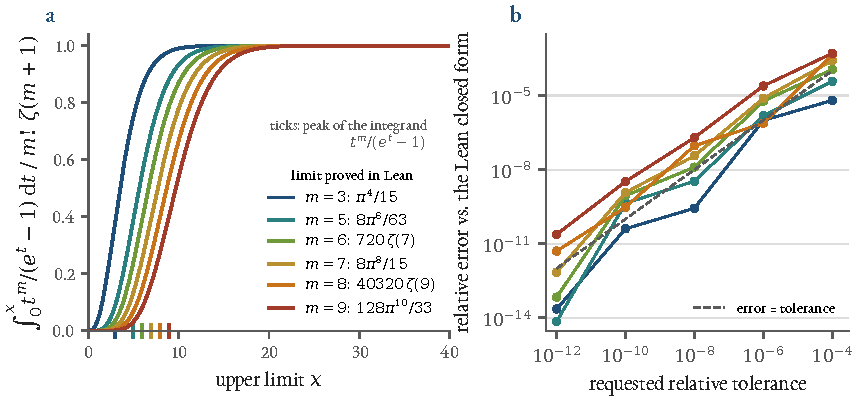
\includegraphics[width=\linewidth]{figures/ch04_bose.pdf}
\caption[The six Bose integrals of the Lean statement, computed by CVODE]{The six Bose integrals of Lean's \lean{bose\_integral\_values} computed by CVODE (Adams). \textbf{(a)} The cumulative integrals $\int_0^x t^m/(e^t-1)\,\mathrm dt$ divided by their limits; the integrand peaks near $t=m$ (ticks), so the higher-order terms of the series draw their weight from higher energies. \textbf{(b)} Relative error against the closed forms proved in Lean, versus the requested relative tolerance; the dashed line is error equal to tolerance.}\label{ch04:fig-bose}
\end{figure}

The largest error is between \cfv{bose-ratio-min} and \cfv{bose-ratio-max} times the requested tolerance over the whole range from $10^{-4}$ to $10^{-12}$ (the global error of a multistep method exceeds its local tolerance); at the tightest tolerance the six closed forms $\pi^4/15$ to $128\pi^{10}/33$ are matched to $\cfv{bose-err-1m12}$ (\cref{ch04:fig-bose}b).
Panel (a) carries a physical point for later: the integrand $t^m/(e^t-1)$ peaks near $t=m$, so the term of order $T^{m}$ draws its weight from phonons of energy about $m\,\cfkB T$, the $L$ term from nine thermal energies, not one: a series in $T$ is a series in progressively less thermal phonons.

\subsection{The thermal integral with no series at all}
Now the experiment that matters.
For the model dispersion, let the solver integrate over wavevector the thermal integral that \emph{defines} the specific heat, with one ODE component per temperature, and compare with the truncated series.
There is one technical step, and it is a use of the first Lean theorem.
Written naively, the answer is of order $A\,T^3$ and the interesting part, the series' corrections, is a small difference of order $T^2$ (relative) hidden inside it; a solver with relative tolerance $10^{-12}$ then sees the corrections only to $10^{-12}$ of the whole.
But the Debye law is \emph{proved}: $\int_0^\infty (V\cfkB/2\pi^2)\,k^2 f(\hbar ck/\cfkB T)\,\mathrm dk=A\,T^3$ exactly (\lean{debye\_specific\_heat}).
So subtract it inside the integrand, and give the solver only the difference:
\begin{align}
 \frac{C_V(T)}{A\,T^3}&=1+\int_0^{k_{\max}}\frac{V\cfkB\,k^2}{2\pi^2\,A\,T^3}\Bigl[f(x_{\rm poly})-f(x_{\rm D})\Bigr]\mathrm dk,\label{ch04:eq-ode}\\
 x_{\rm poly}&=\frac{\hbar c\,k(1+\alpha_2k^2+\alpha_3k^3+\alpha_4k^4)}{\cfkB T},\qquad x_{\rm D}=\frac{\hbar ck}{\cfkB T},\nonumber
\end{align}
with $f(x)=x^2e^x/(e^x-1)^2$ and $k_{\max}=2.5\ \cfAng^{-1}$ (beyond it the Debye integrand contributes less than $10^{-14}$ of $A\,T^3$ for every $T\le1\cfK$).
The right-hand side of the ODE is the integrand of \eqref{ch04:eq-ode} evaluated at all the temperatures at once.

\begin{rustbox}{CVODE: the specific heat of the model dispersion, no series}
\begin{lstlisting}[style=py,basicstyle=\ttfamily\footnotesize]
def rhs_model(k, y):               # one component per temperature in T_all (68 of them)
    if k <= 0.0:
        return [0.0]*len(T_all)
    xp = cc.THETA*cc.u_poly(k)/T_all          # eps/k_B T, polynomial dispersion
    xd = cc.THETA*k/T_all                     # eps/k_B T, Debye dispersion
    return (cc.PREF*k*k*(cc.bose_weight(xp) - cc.bose_weight(xd))/fT(T_all)).tolist()
# excerpt of figures/ch04_cvode_compute.py;  cc.PREF = V k_B/(2 pi^2),  fT(T) = A T^3
y, info = solve_ode(rhs_model, [0.0]*len(T_all), [0.0, cc.KMAX_MODEL],
                    1e-12, 1e-14, "model")
\end{lstlisting}
\noindent \emph{\cfv{nT-all} temperatures (\cfv{nT-log} geometrically spaced from $0.005$ to $1\cfK$, the reference temperature $0.02\cfK$, and the \cfv{nT-lin} of the measured table), Adams, relative tolerance $10^{-12}$, absolute $10^{-14}$ in units of $A\,T^3$: \cfv{model-calls} right-hand-side calls, \cfv{model-seconds} s on the shared 8-core machine at load average about \cfv{model-load}. Against a 30-digit \texttt{mpmath} quadrature of the same integrand at seven temperatures ($0.005$ to $1\cfK$) the absolute error is \cfv{model-abserr-0.1} at $0.1\cfK$ and at most \cfv{model-abserr} (at $0.005\cfK$). Without the subtraction, at the same tolerances: \cfv{model-raw-abserr-0.1} at $0.1\cfK$.}
\end{rustbox}

The subtraction is worth having: at relative tolerance $10^{-8}$ it reduces the absolute error of the result from \cfv{raw8-0.005} to \cfv{sub8-0.005} at $0.005\cfK$ and from \cfv{raw8-0.1} to \cfv{sub8-0.1} at $0.1\cfK$.
The proved Debye law is not decoration here, it is what lets the solver see the series.

\begin{figure}[t]\centering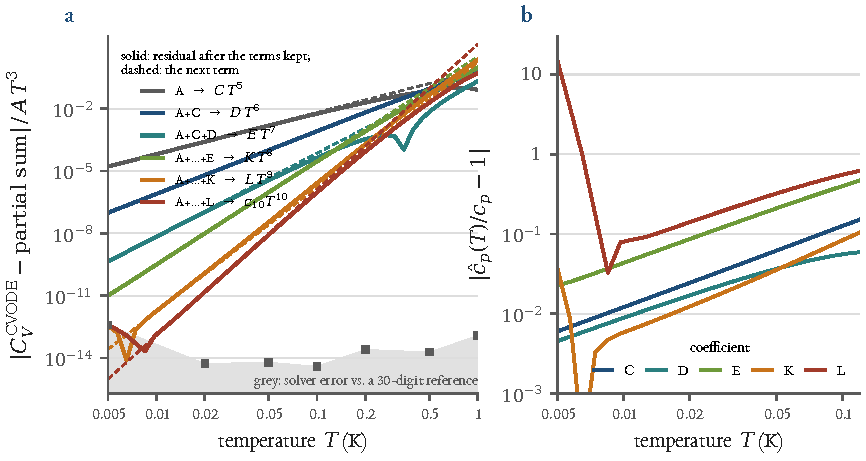
\includegraphics[width=\linewidth]{figures/ch04_ladder.pdf}
\caption[The solver against the proved series]{The solver against the proved series. \textbf{(a)} The absolute difference between the CVODE value of $C_V/A\,T^3$ for the model dispersion and the truncation of Eq.~(22) named on each line, versus $T$ (solid), with the next term of the series (dashed): each line should have the slope of the term it does not contain. The grey squares are the solver's own absolute error, measured against a 30-digit reference at seven temperatures. The top line (only $A$) is Debye's law; the bottom line (after $L$) is compared with a coefficient, $c_{10}$, that Lean does not contain and exact rational arithmetic supplies. \textbf{(b)} The relative error of the coefficient that the numerical data themselves suggest, $\hat c_p(T)=(C_V-\sum_{q<p}c_qT^q)/T^p$ with the coefficients $c_q$ ($q<p$) of Eq.~(22), against $c_p$.}\label{ch04:fig-ladder}
\end{figure}

\Cref{ch04:fig-ladder}a is the test.
If the closed forms are the coefficients, then the residual after $A$ is $C\,T^5(1+O(T))$, that after $A+C$ is $D\,T^6(1+O(T))$, and so on: a ladder of straight lines in logarithmic axes, with slopes $2,3,4,5,6$ (the powers of $T$ minus 3) and a last line of slope $7$.
The lines are straight, and the fitted slopes agree with the expected ones to within about \cfv{slope-maxdev} (the slope of a sum of two power laws is not exactly that of the leading one).
Over the range where each residual lies above a thousand times the solver's error and $T\le0.06\cfK$, fitted slopes against the expected ones are:
\begin{center}\small
\begin{tabular}{@{}lcccccc@{}}\toprule
 truncated after & $A$ & $A{+}C$ & $A{+}C{+}D$ & $\dots{+}E$ & $\dots{+}K$ & $\dots{+}L$\\ \midrule
 next term & $C\,T^5$ & $D\,T^6$ & $E\,T^7$ & $K\,T^8$ & $L\,T^9$ & $c_{10}T^{10}$\\
 expected slope & \cfv{slope-exp-A} & \cfv{slope-exp-AC} & \cfv{slope-exp-ACD} & \cfv{slope-exp-ACDE} & \cfv{slope-exp-ACDEK} & \cfv{slope-exp-ACDEKL}\\
 fitted slope & \cfv{slope-A} & \cfv{slope-AC} & \cfv{slope-ACD} & \cfv{slope-ACDE} & \cfv{slope-ACDEK} & \cfv{slope-ACDEKL}\\
 residual / next term at the lowest $T$ & \cfv{ratio-A} & \cfv{ratio-AC} & \cfv{ratio-ACD} & \cfv{ratio-ACDE} & \cfv{ratio-ACDEK} & \cfv{ratio-ACDEKL}\\ \bottomrule
\end{tabular}
\end{center}
The solid lines meet the dashed ones as $T\to0$: at the lowest temperature of each line the residual is within about 10 per cent of the next term (last row), and the solver's absolute error, in units of $A\,T^3$, is $\cfv{floor-0.1}$ at $0.1\cfK$ (grey squares in the figure).
The absence of a $T^4$ term, the exactness of $A,C,D,E,K$ and the order of $L$ are thus visible in a computation that never used a series.
The one coefficient \emph{not} confirmed by Lean here, $c_{10}$, is confirmed by the solver to the same standard --- as it should be, since exact rational arithmetic computed it.

\subsection{What numerics cannot see}
A solver is blind below its tolerance, and the series makes that blindness worse.
\Cref{ch04:fig-ladder}b asks how well the numerical data alone would determine each coefficient.
The quantity $\hat c_p(T)=(C_V-\sum_{q<p}c_qT^q)/T^p$ tends to $c_p$ as $T\to0$, but only linearly (the first neglected term enters as $c_{p+1}T/c_p$), and the smaller $T$, the more of $\hat c_p$ is solver noise divided by $T^p$.
At $0.02\cfK$, with data whose absolute error in units of $A\,T^3$ is only $\cfv{floor-0.02}$, the coefficients $C,D,E,K,L$ come out with relative errors of $\cfv{rec-0.02-C}$, $\cfv{rec-0.02-D}$, $\cfv{rec-0.02-E}$, $\cfv{rec-0.02-K}$ and $\cfv{rec-0.02-L}$ per cent against the Lean values; at $0.05\cfK$ of $\cfv{rec-0.05-C}$, $\cfv{rec-0.05-D}$, $\cfv{rec-0.05-E}$, $\cfv{rec-0.05-K}$ and $\cfv{rec-0.05-L}$ per cent.
This is the inverse problem of an experimenter who fits $C_V/T^3$ to a polynomial: the forward map from the dispersion to the series is explicit and well conditioned, the inverse map is not.

It also explains why two of the four wrong versions of the previous section could not have been caught numerically.
Replacing $15120$ by $15121$ changes $C_V/A\,T^3$ at $0.1\cfK$ by $\cfv{ctl-D-0.1}$ and replacing $55$ by $54$ by $\cfv{ctl-L-0.1}$, whereas the first term the series does not contain, $c_{10}T^{10}$, contributes $\cfv{ctl-next-0.1}$, that is $\cfv{ctl-D-ratio}$ and $\cfv{ctl-L-ratio}$ times more.
Both effects are far above the solver's error ($\cfv{floor-0.1}$), but cannot be separated from the next term of the series without already knowing it.
The coarser slip $8\alpha_2\alpha_3$ for $9\alpha_2\alpha_3$ in $K$ changes $C_V/A\,T^3$ by $\cfv{ctl-K-0.1}$, $\cfv{ctl-K-ratio}$ times the neighbouring term; it would turn the slope-6 line of \cref{ch04:fig-ladder}a into a line of slope 5, and the solver would catch it.
Lean rejected all of them.
The two instruments are not redundant: the solver sees a whole function, its slopes and gross slips; the proof assistant sees every coefficient to the last digit.


%% ====================================================================================================================
\section{The series meets the measured curve}\label{ch04:sec-data}

Everything so far concerned a \emph{model}, the polynomial \eqref{ch04:eq-disp}.
The specific heat of helium is the integral \eqref{ch04:eq-energy} of the \emph{measured} dispersion.
This section puts the two next to each other, with one rule: nothing is tuned.
The coefficients, $c$ and $V$ are those quoted in the paper, and the dispersion is the open table.

\subsection{Reproducing the paper's table}
The open ancillary files of the paper contain, besides the dispersion, a table of the specific heat from $0.01$ to $1.3\cfK$ with three columns: total, ``phonon'' and ``roton''.
I recomputed it from the dispersion table with CVODE: the table interpolated by a cubic spline in $k$, the thermal integral written as an initial-value problem in $k$ with one component per temperature (as in Section~\ref{ch04:sec-solver}), integrated first to the maxon wavevector $k_M=\cfv{maxon-k}\ \cfAng^{-1}$ (the maximum of the table's $\varepsilon(k)$: the phonon column) and then to the end of the table at $3.6\ \cfAng^{-1}$ (the total), for the \cfv{n-T} temperatures $0.05,0.10,\dots,1.30\cfK$.
Adams, relative tolerance $10^{-8}$, absolute $10^{-11}$ in units of $A\,T^3$; \cfv{repro-calls} right-hand-side evaluations in about \cfv{repro-seconds} s on the shared machine (load average $\approx\cfv{repro-load}$).
Against the tabulated total the relative difference is at worst $\cfv{repro-max}$ (at $\cfv{repro-T-of-max}\cfK$) and \cfv{repro-median} in the median; the phonon column agrees to $\cfv{repro-ph-max}$; SciPy's adaptive quadrature gives the same integral as CVODE to $\cfv{repro-vs-quad}$.
The table carries four significant digits, which would show differences of order $10^{-4}$; the larger differences are real but small compared with the table's own uncertainty column ($\cfv{paper-unc-0.7}$ per cent at $0.7\cfK$), and I did not track them down (the interpolation between grid points and the treatment of the ultrasound-based region below $0.15\ \cfAng^{-1}$ are candidates).
It is a reproduction of a tabulated number from its own open data, nothing more; but it tells us that the integral computed below is the same quantity as the table's.

\subsection{Which excitations carry the heat}
\begin{figure}[t]\centering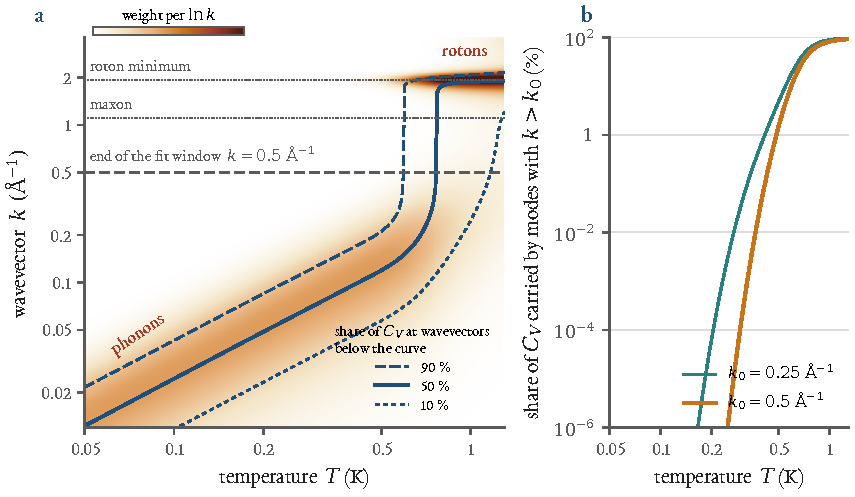
\includegraphics[width=\linewidth]{figures/ch04_heatmap.pdf}
\caption[Which excitations carry the heat?]{Which excitations carry the heat? \textbf{(a)} The distribution of the specific heat over the wavevector $k$ of the excitation, $w(k,T)=\bigl(V\cfkB/2\pi^2\bigr)k^2 f(\varepsilon/\cfkB T)/C_V(T)$ with $f(x)=x^2e^x/(e^x-1)^2$, per unit $\ln k$, computed from the measured dispersion table (integration limit $3.6\ \cfAng^{-1}$); white is no weight. The phonon ridge climbs along $k\propto T$; at about $0.8\cfK$ the median wavevector jumps to the roton minimum. Curves: wavevectors below which 10, 50 and 90 per cent of $C_V$ sit. \textbf{(b)} The share of $C_V$ carried by modes with $k>k_0$, for $k_0=0.25$ and $0.5\ \cfAng^{-1}$.}\label{ch04:fig-heatmap}
\end{figure}

\Cref{ch04:fig-heatmap} is built from the same table.
It shows the structure that the series ignores.
At $0.1\cfK$ half of the specific heat is carried by phonons with $k<\cfv{med-k-0.1}\ \cfAng^{-1}$, wavelengths longer than $\cfv{lambda-0.1}\ \cfAng$, and nine tenths by $k<\cfv{q90-k-0.1}\ \cfAng^{-1}$; at $0.5\cfK$ the numbers are $\cfv{med-k-0.5}$ and $\cfv{q90-k-0.5}\ \cfAng^{-1}$.
The ridge is a straight line of unit slope in these logarithmic axes, as the Debye law says ($k\propto T$), bending slowly because $\alpha_2>0$.
Then the weight switches: in my integration the roton part of the integral overtakes the phonon part at $\cfv{T-cross}\cfK$, and the median wavevector jumps to the roton minimum at $k=\cfv{roton-k}\ \cfAng^{-1}$.
Panel (b) quantifies what the polynomial's range of validity would suggest.
If the polynomial is only trusted below $0.5\ \cfAng^{-1}$, the fraction of the specific heat that falls outside it is $\cfv{share05-0.3}$ per cent at $0.3\cfK$, $\cfv{share05-0.5}$ per cent at $0.5\cfK$, $\cfv{share05-0.7}$ per cent at $0.7\cfK$ and $\cfv{share05-1.0}$ per cent at $1\cfK$.
So by this criterion the polynomial should serve almost to $0.5\cfK$ and fail within a few tenths of a kelvin above.
We now see whether the series does.

\subsection{An error budget}
\begin{figure}[t]\centering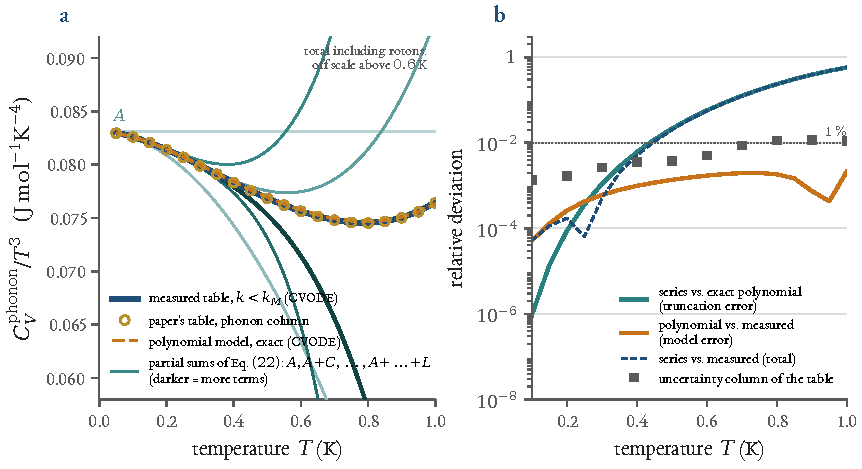
\includegraphics[width=\linewidth]{figures/ch04_budget.pdf}
\caption[Eq.~(22) against the integral of the measured dispersion]{Eq.~(22) against the integral of the measured dispersion. \textbf{(a)} $C_V/T^3$ of the phonon part ($k<k_M$): the integral of the measured table (blue, CVODE), the paper's own table column (circles), the exact integral of the polynomial model (orange dashed, CVODE), and the partial sums of Eq.~(22) (teal, darkening with the number of terms). The total including rotons rises above the frame beyond $0.6\cfK$. \textbf{(b)} Three relative deviations: the six-term series against the exact integral of the \emph{same} polynomial (the series' own truncation error, teal); that polynomial against the measured table (the model error, orange); the series against the measured table (the total, blue dashed). Grey squares: the uncertainty column of the paper's table, relative to its total $C_V$.}\label{ch04:fig-budget}
\end{figure}

\Cref{ch04:fig-budget} separates two sources of error that are usually mixed.
The six-term series is an approximation to the integral of the polynomial, and the polynomial is an approximation to helium.
The solver gives the exact integral of the polynomial, so the two can be told apart.
Up to about $0.3\cfK$ everything is excellent: the series differs from the exact polynomial integral by $\cfv{bud-trunc-pct-0.3}$ per cent at $0.3\cfK$, and the polynomial differs from the measured phonon integral by $\cfv{bud-model-pct-0.3}$ per cent.
At $0.5\cfK$ the picture has changed: the model error is $\cfv{bud-model-pct-0.5}$ per cent and the truncation error of the six terms is $\cfv{bud-trunc-pct-0.5}$ per cent, more than a factor of ten larger.
At $0.7\cfK$ the truncation error has reached $\cfv{bud-trunc-pct-0.7}$ per cent; above that the series is useless as an approximation.
The six-term series first departs from the exact polynomial integral by more than one per cent at $\cfv{bud-first_T_series6_vs_poly_exceeds_1pct}\cfK$.
For scale, the uncertainty column of the paper's table is $\cfv{paper-unc-0.1}$ per cent of the total at $0.1\cfK$, $\cfv{paper-unc-0.3}$ per cent at $0.3\cfK$ and $\cfv{paper-unc-0.5}$ per cent at $0.5\cfK$ (grey squares).
So the limit on the series is not the polynomial's range of validity, as the heat map suggested --- at $0.5\cfK$ only $\cfv{share05-0.5}$ per cent of the heat is carried outside it --- but the \emph{series} itself: as a series in $T$ it runs out of accuracy earlier than the model it expands.

\subsection{A series that does not converge}
\begin{figure}[t]\centering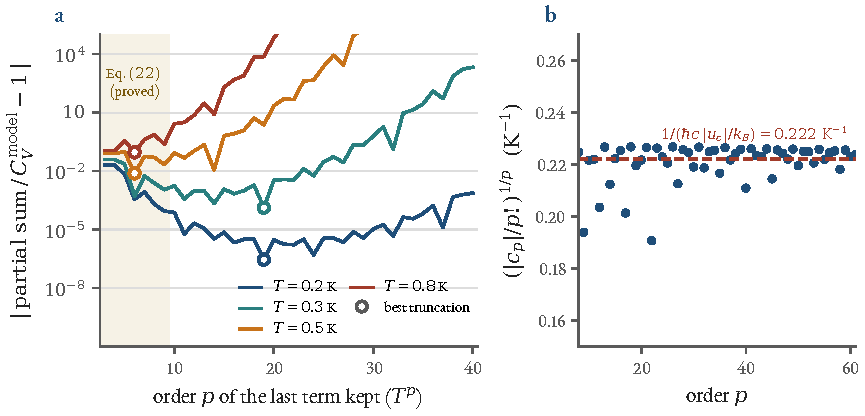
\includegraphics[width=\linewidth]{figures/ch04_asymptotic.pdf}
\caption[The series is asymptotic, not convergent]{The series continues to every order and is asymptotic, not convergent. \textbf{(a)} Relative error of the partial sum through $T^p$ against the exact (CVODE) integral of the polynomial model, for four temperatures, with the coefficients of Eq.~(22) and beyond from exact rational arithmetic; circles mark the best truncation. The gold band is the range proved in Lean. \textbf{(b)} The root test $(|c_p|/p!)^{1/p}$ of the coefficients $c_p$ of $T^p$; the dashed line is $1/(\hbar c|u_c|/\cfkB)$, computed from the critical points of $u(k)$ alone.}\label{ch04:fig-asymptotic}
\end{figure}

The exact-rational script of Section~\ref{ch04:sec-confirm} does not stop at $L$.
For the paper's coefficient set the coefficients of $T^p$ for $p=3,5,6,7,8,9$ are, relative to $A$: $1$, $\cfv{rA-5}$, $\cfv{rA-6}$, $\cfv{rA-7}$, $\cfv{rA-8}$, $\cfv{rA-9}$, and the next ones, beyond Lean, are $\cfv{rA-10}$ ($p=10$), $\cfv{rA-11}$, $\cfv{rA-12}$, $\cfv{rA-13}$, $\cfv{rA-14}$, growing.
\Cref{ch04:fig-asymptotic}a shows the consequence.
At $T=0.2\cfK$ the error of the partial sum falls as terms are added, reaches $\cfv{best-err-0.2}$ at order $p=\cfv{best-order-0.2}$, and then grows without bound; at $0.3\cfK$ the best is $\cfv{best-err-0.3}$ (order $\cfv{best-order-0.3}$); at $0.5\cfK$ it is $\cfv{best-err-0.5}$ (order $\cfv{best-order-0.5}$); at $0.8\cfK$ it is $\cfv{best-err-0.8}$ (order $\cfv{best-order-0.8}$).
So the six terms of Eq.~(22), through $T^9$, stop well short of the best truncation at $0.2$ and $0.3\cfK$, and overshoot it from $0.5\cfK$ on: at $0.5\cfK$ the error after $A+C+D$ ($T^6$) is $\cfv{best-err-0.5}$, smaller than the $\cfv{err9-0.5}$ after all six terms.
The six terms of Eq.~(22) are the beginning of an \emph{asymptotic} expansion, not of a convergent one that could be extended at will; its best truncation depends on the temperature.

Where does the divergence come from?
Two factors.
The Bose integrals contribute $(n+2)!$ to the coefficient of $T^{n+1}$ (they are $\Gamma$ functions), a factorial.
And the density of states $g(u)=\sum g_nu^n$ has a finite radius of convergence: $k(u)$ is the inverse function of $u(k)$ and has a branch point at every critical value of $u(k)$, where $\mathrm du/\mathrm dk=0$, so $g_n$ grows like $R^{-n}$ with $R$ the distance from the origin to the nearest singularity on the principal sheet.
The polynomial $u(k)=k(1+\alpha_2k^2+\alpha_3k^3+\alpha_4k^4)$ has degree five, so $\mathrm du/\mathrm dk=0$ is a quartic equation, with two complex-conjugate pairs of roots; the pair with the smaller critical value sits at $k_c=\cfv{uc-k-re}\pm\cfv{uc-k-im}\,i\ \cfAng^{-1}$ and gives $u_c=\cfv{uc-u-re}\pm\cfv{uc-u-im}\,i\ \cfAng^{-1}$, $|u_c|=\cfv{uc-abs}\ \cfAng^{-1}$, that is an energy $\hbar c|u_c|/\cfkB=\cfv{uc-K}\cfK$.
Together: the coefficient of $T^p$ behaves like $p!\,(\hbar c|u_c|/\cfkB)^{-p}$, and the root test $(|c_p|/p!)^{1/p}$ should tend to $1/(\hbar c|u_c|/\cfkB)=\cfv{uc-inv}\ \mathrm{K^{-1}}$.
\Cref{ch04:fig-asymptotic}b shows that it does: the sequence is $\cfv{root-p20}$ at $p=20$, $\cfv{root-p40}$ at $p=40$ and $\cfv{root-p60}$ at $p=60$.
The same reasoning gives the optimal order, where the factorial overtakes the geometric decay, $p^\ast\approx\hbar c|u_c|/\cfkB T$, and the best accuracy, $\exp(-\hbar c|u_c|/\cfkB T)$ times a power of $T$.
The order $p^\ast$ at which the terms (taken as the largest of three consecutive ones, to suppress accidental zeros) are smallest is $\cfv{pstar-0.1}$ at $0.1\cfK$ (the estimate gives $\cfv{pstar-pred-0.1}$), $\cfv{pstar-0.2}$ at $0.2\cfK$ ($\cfv{pstar-pred-0.2}$), $\cfv{pstar-0.3}$ at $0.3\cfK$ ($\cfv{pstar-pred-0.3}$) and $\cfv{pstar-0.4}$ at $0.4\cfK$ ($\cfv{pstar-pred-0.4}$); and fitting the size of those smallest terms for $\cfv{fit-T-lo}\le T\le\cfv{fit-T-hi}\cfK$ to $a\,T^s e^{-b/T}$ gives $b=\cfv{fit-b}\cfK$ and $s=\cfv{fit-s}$, against the predicted $b=\cfv{fit-b-pred}\cfK$.
The $\cfv{uc-K}\cfK$ scale is a property of the \emph{polynomial} --- the complex critical points are an artefact of truncating the dispersion at $\alpha_4$ --- and not of helium, whose measured dispersion has a real maxon at $\varepsilon/\cfkB=\cfv{maxon-K}\cfK$ and a roton minimum at $\cfv{roton-K}\cfK$; it is an illustration of how a truncated polynomial and a Bose integral conspire, not a statement about the real fluid.
What the figure says is limited: below about $0.3\cfK$ the six-term series represents the integral of the polynomial excellently, above $0.5\cfK$ it does not, and the transition is set by the mathematics of the series, not by the measured curve.


%% ====================================================================================================================
\section{What this chapter establishes, and what it does not}\label{ch04:sec-honest}

\begin{honestbox}
\textbf{Proved in Lean (statements about mathematics).}
(i) $\int_0^\infty t^n/(e^t-1)\,\mathrm dt=n!\,\zeta(n+1)$ for all $n\ge1$, and its six values at $s=4,6,7,8,9,10$.
(ii) The inverse series printed in the paper inverts $u=k(1+\alpha_1k+\dots+\alpha_6k^6)$ modulo $u^8$, and $k^2\,\mathrm dk/\mathrm du$ equals the density-of-states polynomial modulo $u^9$.
(iii) The derivative with respect to $T$ of the term-by-term energy is the six closed forms $A,C,D,E,K,L$ of Eq.~(22).
(iv) New in this book: the density-of-states brackets are literally the coefficients of $k^2\cdot k'$, with $k'$ the formal derivative, and the capstone can be stated with them and with the Mellin transforms, nothing retyped, and with the energy of each monomial written as its integral (Section~\ref{ch04:sec-newlean}).

\textbf{Derived independently, not in Lean.} The same coefficients by computer algebra, and by exact rational arithmetic, which also gives the terms beyond $L$.

\textbf{Computed here with rusty-SUNDIALS (CVODE, Adams, commit \cfv{rs-commit-short}).} The Bose integrals to the tolerance requested; the specific heat of the model dispersion with no series, whose residual after each truncation has the slope of the next term; the integral of the measured dispersion table, reproducing the paper's table to $\cfv{repro-max}$ (relative, maximum over $0.05$--$1.3\cfK$).

\textbf{Measured by others and used as given.} The dispersion relation $\varepsilon(k)$ (neutron scattering, open ancillary data) and the paper's numerical specific heat, which is itself an integral of that dispersion. I did not measure anything, and I did not compare with calorimetry: the calorimetric data are not in the open files.

\textbf{Not established, and not claimed.}
(a) That Eq.~(22) describes liquid helium at any temperature: it is a statement about the polynomial \eqref{ch04:eq-disp}. Section~\ref{ch04:sec-data} shows what the six terms do, for the model and against the table.
(b) That the series converges: for the model it does not, and the divergence is computed here, not proved in Lean. The legitimacy of term-by-term integration, and the asymptotic character of the expansion for a measured curve, are analytical statements that the library does not contain.
(c) Anything about $\alpha_1\ne0$ (the $T^4$ term and the $\alpha_1$-dependence of the other coefficients): the Lean files treat $C_V$ for $\alpha_1=0$ only.
(d) Anything about errata in the paper. The check found no discrepancy between the printed closed forms and the derived ones; the formulas checked are those of the arXiv version, and the version of record was not compared.
(e) The picture of a gas of non-interacting phonons, and the density of states $V k^2\mathrm dk/2\pi^2$, are modelling assumptions of the physics; no theorem here proves that liquid helium is such a gas.

\textbf{What failed or was left unexplained.}
The first version of the new Lean file forgot \lean{open Real}: Lean then read \lean{π} as a fresh variable (an auto-bound implicit), and the capstone failed with a type mismatch between that variable and \lean{Real.pi} --- the checker rejecting a statement about the wrong object, as it should.
My first runs used a stale build of the solver, whose Adams method was implicit Euler: plausible numbers, wrong by up to hundreds of times the tolerance; they were discarded, and every number of the chapter was recomputed with the fixed build (Section~\ref{ch04:sec-solver}).
The derivation check of 2026-09-21 was not pre-registered; the design note records that lapse.
\end{honestbox}

%% ====================================================================================================================
\section*{Exercises}\addcontentsline{toc}{section}{Exercises}

\paragraph{Exercise 1.}
\emph{The missing $T^4$ term.} Keep $\alpha_1\neq0$ and set $\alpha_2=\alpha_3=\dots=0$, so that $\varepsilon=\hbar ck(1+\alpha_1k)$.
(a) Invert $u=k(1+\alpha_1k)$ exactly and show that the density of states is $k^2\,\mathrm dk/\mathrm du=u^2-4\alpha_1u^3+15\alpha_1^2u^4-56\alpha_1^3u^5+\dots$.
(b) Use \eqref{ch04:eq-series} with $n=3$ to show that $C_V$ acquires a term $B\,T^4$ with $B=-240\,\zeta(5)\,\alpha_1\,V\cfkB^5/(\pi^2\hbar^4c^4)$.
(c) Explain why Eq.~(22) has no such term, and which line of \lean{density\_of\_states} is the $T^4$ term's absence.\\
\emph{Hint.} (a) $k=(-1+\sqrt{1+4\alpha_1u})/2\alpha_1$, and $g=\mathrm d(k^3/3)/\mathrm du$. (b) The factor is $(n+2)!\,\zeta(n+2)=5!\,\zeta(5)$ and $g_3=-4\alpha_1$. (c) $g_3=0$ when $\alpha_1=0$; the missing $e^3$ in the right-hand side. The expression in (b) agrees with the $B$ printed for $\alpha_1\ne0$ in the Supplemental Material of the arXiv version of the paper; the Lean files do not cover it.

\paragraph{Exercise 2.}
\emph{Where do $5$, $28$, $165$ come from?} Set $\alpha_3=\alpha_4=\alpha_5=\alpha_6=0$.
Show, by Lagrange inversion, that $g_{2n+2}=(-1)^n\binom{3n+2}{n}\alpha_2^n$.
Check it against the brackets of $C$, $E$ and $L$ ($-5$, $28=7\cdot4$, $-165=-3\cdot55$), and predict the coefficient $1001\,\alpha_2^4$ of $u^{10}$.\\
\emph{Hint.} For $u=k(1+\alpha_2k^2)$ one has $[u^m]\,k^r=\tfrac rm\,[k^{m-r}]\,(1+\alpha_2k^2)^{-m}$. Take $r=3$, $m=2n+3$, and note $g_{2n+2}=\tfrac{2n+3}3\,[u^{2n+3}]\,k^3$. (The formula was checked symbolically through $n=4$ while writing this chapter.)

\paragraph{Exercise 3.}
\emph{Optimal truncation.} At fixed $T$ the terms $c_pT^p$ of the series \eqref{ch04:eq-series} first shrink and then grow.
Using $(|c_p|/p!)^{1/p}\to1/(\hbar c|u_c|/\cfkB)$ with $\hbar c|u_c|/\cfkB=\cfv{uc-K}\cfK$ (Section~\ref{ch04:sec-data}), show that the smallest term sits near $p^\ast\approx\cfv{uc-K}\cfK/T$ and that the best accuracy of the truncated series is of order $\exp(-\cfv{uc-K}\cfK/T)$ up to a power of $T$.
Compare with \cref{ch04:fig-asymptotic} and Section~\ref{ch04:sec-data}: at $T=0.2\cfK$ the smallest terms sit at order $\cfv{pstar-0.2}$ while the estimate gives $\cfv{pstar-pred-0.2}$.\\
\emph{Hint.} Stirling: $\ln(p!\,x^p)\approx p\ln(px/e)$ with $x=T/\cfv{uc-K}\cfK$; minimize over $p$.

%% ====================================================================================================================
\section*{Notes and further reading}\addcontentsline{toc}{section}{Notes and further reading}

The phonon--roton spectrum is Landau's \cite{Landau1941}; textbook accounts of the quasiparticle picture are in \cite{PitaevskiiStringari2016,Donnelly1991}.
The measurement and the analytical and numerical thermodynamics of this chapter are those of Godfrin and collaborators \cite{Godfrin2021}; the wider survey of excitation spectra of quantum fluids is \cite{GodfrinKrotscheck2022}.
Calorimetric determinations of the phonon dispersion of liquid $^4$He are \cite{Phillips1970,Greywall1978}.
For asymptotic series and the idea of optimal truncation (Section~\ref{ch04:sec-data}) see \cite{BenderOrszag1999}.
The Lean library is \cite{Callens2026lib}, built on Mathlib \cite{Mathlib2020} and Lean~4 \cite{deMoura2021}; the history of the three modules, including the derivation script and the generator of the certificates, is in \texttt{docs/designs/PHONON\_SERIES\_A\_TO\_L.md} of the repository.
The solver is CVODE of the SUNDIALS family \cite{Hindmarsh2005}, in its rusty-SUNDIALS port.
Every figure is made by a script \texttt{figures/ch04\_*.py} from \texttt{ch04\_cvode\_raw.json}, \texttt{ch04\_cvode\_results.npz} and \texttt{ch04\_numbers.json}; every computed number in the text is read from the last of these by \texttt{figures/ch04\_numbers\_tex.py}.
